\documentclass[frames,pdf,slideColor,colorBG,accumulate,total]{prosper}
\usepackage[francais]{babel}
\usepackage{amsmath, amsfonts, amsbsy, pstricks, pst-node, pst-text, pst-3d}
\usepackage{slashbox}
\usepackage{moreverb,epsfig,color,subfigure}
\NoFrenchBabelItemize
\usepackage{ucs}
\usepackage[utf8x]{inputenc}
\usepackage{graphicx,color,caption2,amssymb,pstricks,lmodern}

\newcommand{\items}[1]{\begin{itemize} \item #1 \end{itemize}}
\newcommand{\itemss}[2]{\begin{itemize} \item #1 \item #2 \end{itemize}}
\newcommand{\itemsss}[3]{\begin{itemize} \item #1 \item #2 \item #3 \end{itemize}}
\newcommand{\itemssss}[4]{\begin{itemize} \item #1 \item #2 \item #3 \item #4 \end{itemize}}
\newcommand{\slidetextsize}{\footnotesize}
%\newcommand{\captionstyle}[1]{\scriptsize \textbf{#1}}

\myitem{1}{\includegraphics[width=.4cm]{red-bullet-on-white}}
\myitem{2}{\includegraphics[width=.4cm]{green-bullet-on-white}}
\myitem{3}{\includegraphics[width=.4cm]{yellow-bullet-on-blue}}
% ==================================
% Start of Commands Used in Document
% ==================================

\DeclareSymbolFontAlphabet{\mathcalold}{symbols}
\newcommand{\mc}[1]{{\ensuremath{\mathcal{#1}}}}
\newcommand{\mco}[1]{{\ensuremath{\mathcalold{#1}}}}
\newcommand{\mr}[1]{{\ensuremath{\mathrm{#1}}}}
\newcommand{\mb}[1]{{\ensuremath{\mathbf{#1}}}}
\newcommand{\bs}[1]{\ensuremath{\boldsymbol{#1}}}
\newcommand{\ie}{\emph{i.e.}}
\newcommand{\Bayes}{Bayes's}
\newcommand{\field}[1]{\mathbb{#1}}
\newcommand{\real}[1]{\ensuremath{{\field{R}}^{#1}}}
\newcommand{\ints}[1]{\ensuremath{{\field{Z}}^{#1}}}
\newcommand{\defas}{\ensuremath{\stackrel{\scriptscriptstyle{\triangle}}{=}}}
\newcommand{\eye}[1]{\mr I_{#1}}
\newcommand{\model}{\mco I}
\newcommand{\pdf}[2][p]{\ensuremath{#1\left(#2\right)}}
\newcommand{\cpdf}[3][p]{\ensuremath{\pdf[#1]{\left.#2\,\right|\,#3}}}
\newcommand{\norm}[3]{\ensuremath{\mco N\left(#1\,\big|\,#2,\,#3\right)}}
\newcommand{\simnorm}[2]{\ensuremath{\sim \mco N\left(#1,\,#2\right)}}
\newcommand{\simIG}[2]{\ensuremath{\sim \mco{IG}\left(#1,\,#2\right)}}
\newcommand{\BSAR}[1]{\ensuremath{\text{BSAR}(#1)}}
\newcommand{\conv}{\ensuremath{\star}}

% ================================
% End of Commands Used in Document
% ================================
\newlength{\MiniPageLeft}
\newlength{\MiniPageRight}


\title{Initiation à la recherche}
\subtitle{Conception et réalisation d’un logiciel interactif de visualisation de pavages 2D/3D}
%\caption{IR}
\author{A.\textsc{Marguerite} R.\textsc{Rincé}}

%\Logo{
\includegraphics[scale=0.40]{img/logouniv.eps}}
\Logo(9,-0.70){
\includegraphics[scale=0.5]{img/logouniv.eps}}



\institution{
  Université de Nantes \\
  2 rue de la Houssinière, \\
  BP92208, F-44322 Nantes cedex 03, FRANCE
  
}


\begin{document}

% make the title slide
\maketitle

\overlays{3}{
  \begin{slide}[Box]{Présentation du \textsc{LINA}}
    \slidetextsize
    \setlength{\MiniPageLeft}{0.4\textwidth}
    \setlength{\MiniPageRight}{\textwidth}\addtolength{\MiniPageRight}{-\MiniPageLeft}
    \begin{minipage}[t]{\MiniPageLeft}
      \begin{figure}[t]
        \begin{center}
          \onlySlide*{1}{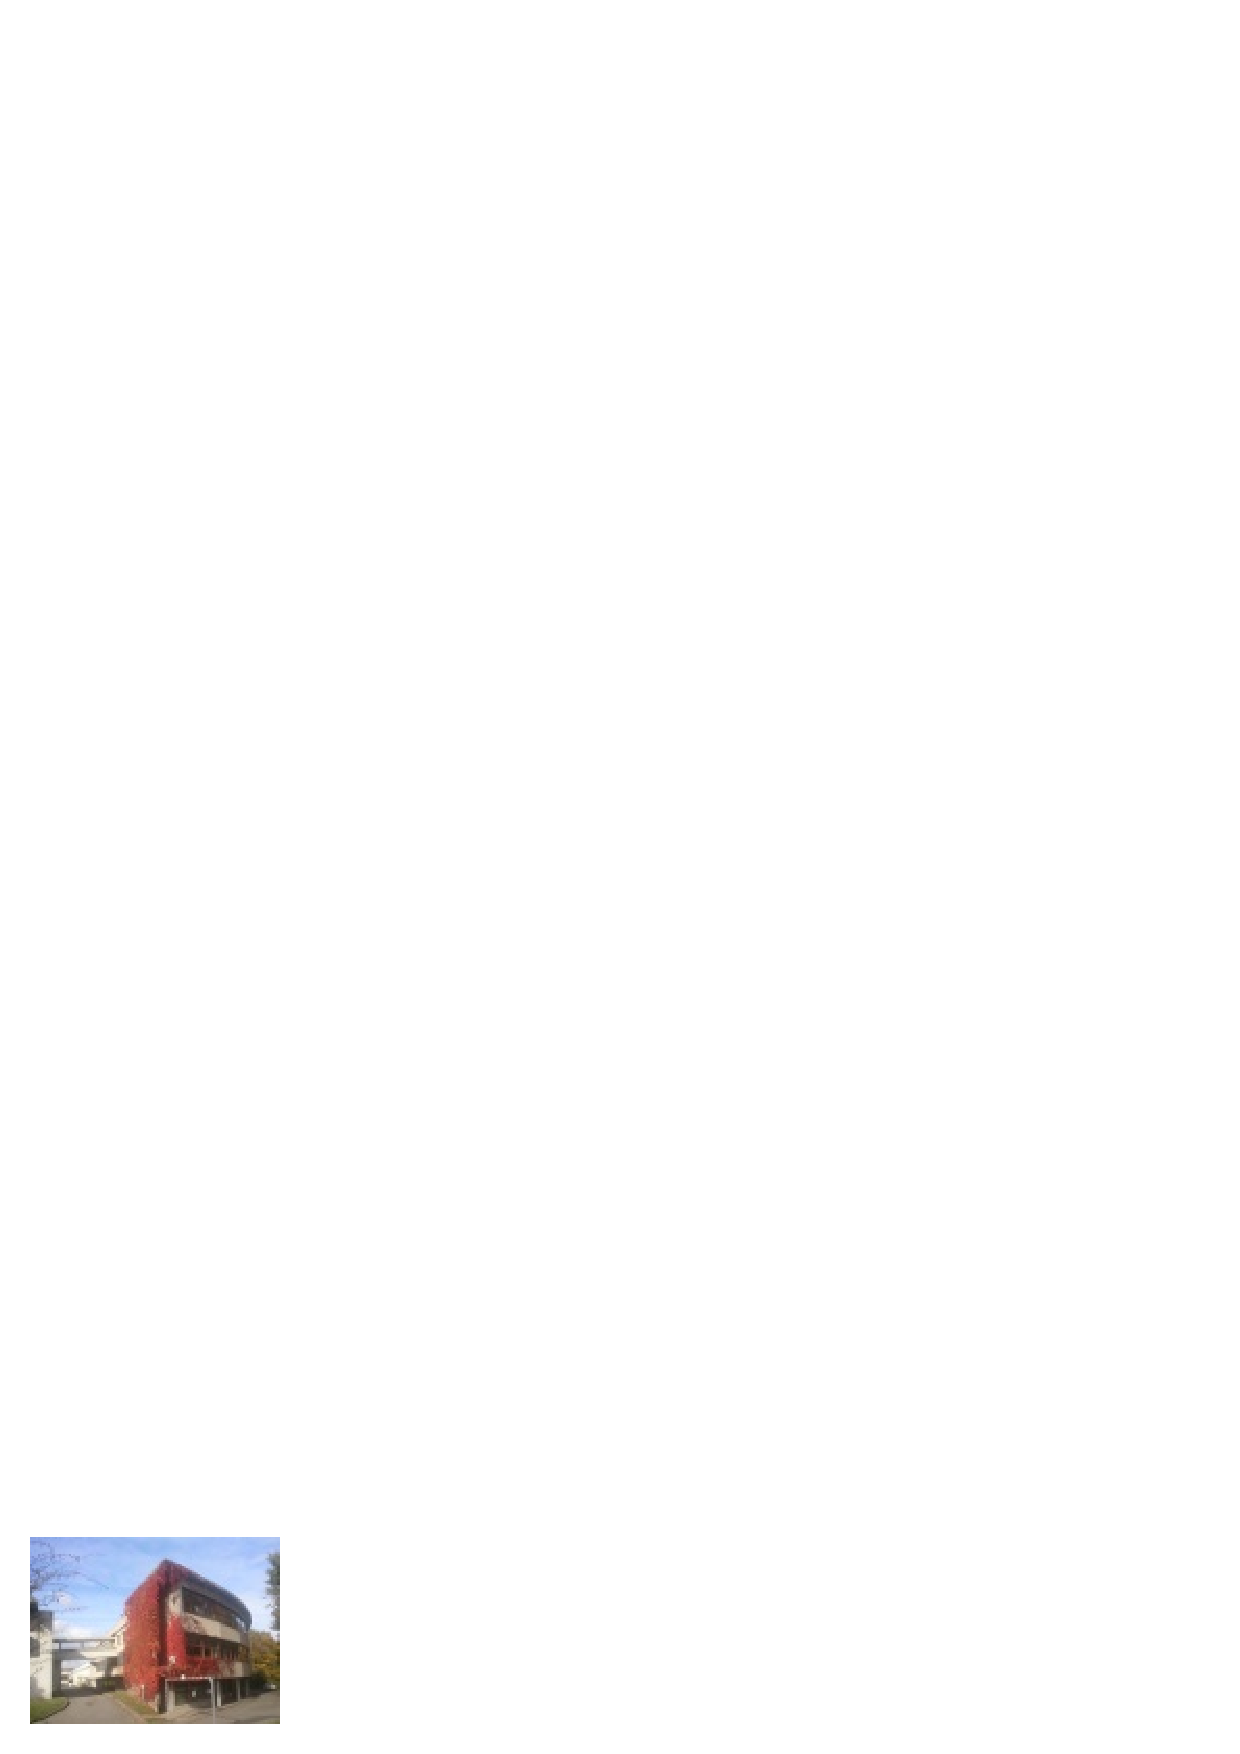
\includegraphics[width=0.8\MiniPageLeft]{img/lina}}
          \fromSlide{2}{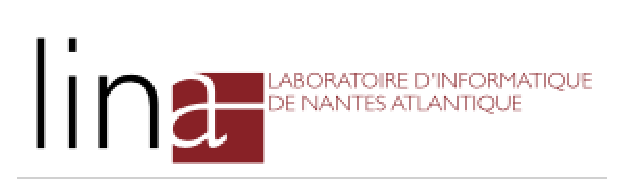
\includegraphics[width=\MiniPageLeft]{img/logolina}}
        \end{center}
      \end{figure}
    \end{minipage}
    \begin{minipage}[t]{\MiniPageRight}
      \begin{Itemize}
      \item Laboratoire d’Informatique de Nantes-Atlantique :
        \begin{Itemize}
        \item Effectif global proche de 170 membres 
          \fromSlide{2}{\item 10 équipes de recherche}
        \end{Itemize}
        \fromSlide{3}{\item Équipe Optimisation globale, optimisation multi-objectifs (\textsc{OPTI})}
      \end{Itemize}
    \end{minipage}
  \end{slide}

%%%%%%%%%%%%%%%%%%%%%%%%%%%%%%%%%%%%%%%%%%%%%%%%%%%%%%%%%%%%%%%%%%%%%%%%%%%%
}\overlays{6}{
  \begin{slide}[Box]{Reprise d'un projet de stage}
    \textbf{Création d'un outil de visualisation}
    \begin{Itemize}
      \fromSlide{1}{\item État d'avancement}
      \begin{Itemize}
        \fromSlide{2}{\item Cahier des charges}
        \fromSlide{3}{\item Document de spécifications}
      \end{Itemize}
      \fromSlide{4}{\item Quelles problématiques à ce stade ?}
      \begin{Itemize}
        \fromSlide{5}{\item Implémenter les entités à visualiser}
        \fromSlide{6}{\item Garantir un affichage fluide}
      \end{Itemize}
    \end{Itemize}
  \end{slide}
}
%%%%%%%%%%%%%%%%%%%%%%%%%%%%%%%%%%%%%%%%%%%%%%%%%%%%%%%%%%%%%%%%%%%%%%%%%%%%
\overlays{9}{
  \begin{slide}[Box]{Problématiques}
    \begin{Itemize}
      \fromSlide{1}{\item Quelle orientation du projet choisir?}
      \begin{Itemize}
        \fromSlide{2}{\item Entamer la conception}
        \fromSlide{3}{\item Effectuer une étude des problématiques de conception }
      \end{Itemize}
      \fromSlide{4}{\item Caractéristiques de l'outil}
      \begin{Itemize}
        \fromSlide{5}{\item Données en entrée}
        \fromSlide{6}{\item Fenêtre de visualisation}
        \fromSlide{7}{\item Dimensions visualisées }
        \fromSlide{8}{\item Filtre}
        \fromSlide{9}{\item Données en sortie}
      \end{Itemize}
    \end{Itemize}
  \end{slide}
}

%% %% %%%%%%%%%%%%%%%%%%%%%%%%%%%%%%%%%%%%%%%%%%%%%%%%%%%%%%%%%%%%%%%%%%%%%%%%%%%%

\overlays{5}{
  \begin{slide}[Box]{Domaine de recherche}
    \slidetextsize
    \textbf{L’Arithmétique des intervalles}\\
    \begin{Itemize} 
      \fromSlide{2}{\item Extension des fonctions aux intervalles}
      \fromSlide{3}{\item Quelques opérations: \\}
    \begin{Itemize}
      \fromSlide{4}{\item Opérateur Plus : \\
        $[a \dots b] + [c \dots d] = [a + c \dots b + d]$ }
      \fromSlide{5}{\item Opérateur Fois : \\
      $ [a \dots b] × [c \dots d] = $\\ \hspace{1cm}$[min(ac, ad, bc, bd) \dots max(ac, ad, bc, bd)]$}
    \end{Itemize}
    \end{Itemize}
    
  \end{slide}
}
%%%%%%%%%%%%%%%%%%%%%%%%%%%%%%%%%%%%%%%%%%%%%%%%%%%%%%%%%%%%%%%%%%%%%%%%%%%%%%%ù
\overlays{4}{
  \begin{slide}[Box]{Domaine de recherche}
    \slidetextsize
    \textbf{Définition d'un \textsc{CSP}}\\
  \begin{Itemize}
    \fromSlide{2}{  \item
      Un ensemble de variables $\mathbf{V} = \left\{ v_1, \dots ,v_n \right\}$.}
    \fromSlide{3}{  \item
      Un domaine de valeurs  $D_i$ pour chaque variable $v_i$  \\ avec $\mathbf{D} =D_1 \times \dots \times D_n $.}
    \fromSlide{4}{  \item
      Un ensemble de contraintes :  $\mathbf{C} = \left\{c_1, \dots ,c_m\right\}$. }
  \end{Itemize}
  \end{slide}
}

\overlays{4}{
  \begin{slide}[Box]{Intersection de 3 cercles}
    \onlySlide*{1}{
      \textbf{Exemple de CSP}
      \begin{figure}[t]
        \begin{center}
          \includegraphics[width=0.45\textwidth]{img/hull.ps}
        \end{center}
      \end{figure}
      \begin{equation*}
        \begin{cases}
          (x-x_{c_1})²+(y-y_{c_1})² = r_{c_1}²\\
          (x-x_{c_2})²+(y-y_{c_2})² = r_{c_2}²\\
          (x-x_{c_3})²+(y-y_{c_3})² = r_{c_3}²
        \end{cases}
      \end{equation*}
}
    \onlySlide*{2}{
    \emph{Hull-consistance} : 1\up{ère} étape
      \begin{figure}[t]
        \begin{center}
          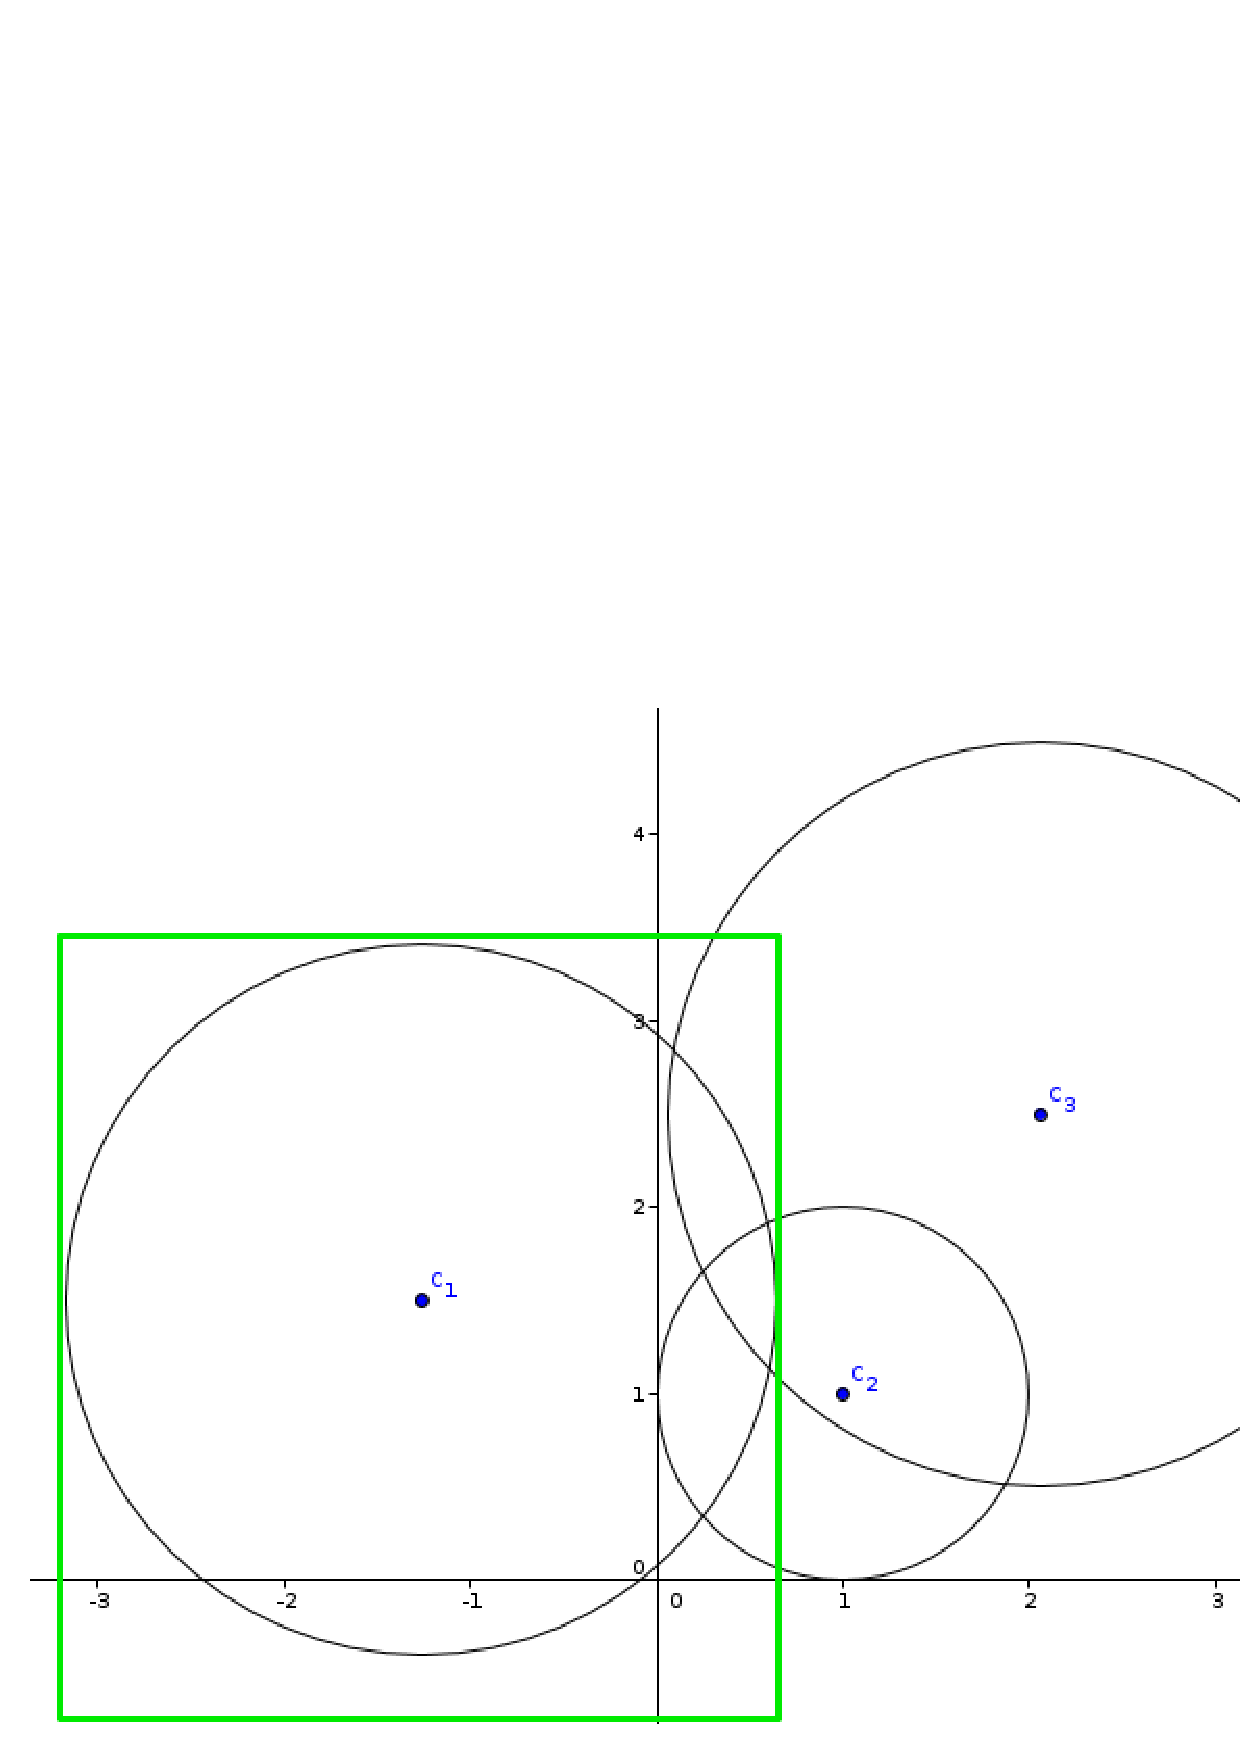
\includegraphics[width=0.55\textwidth]{img/hull1}
        \end{center}
      \end{figure}
      \begin{equation*}
        (x-x_{c_1})²+(y-y_{c_1})² = r_{c_1}²
      \end{equation*}
        }
    \onlySlide*{3}{
    \emph{Hull-consistance} : 2\up{nd} étape
      \begin{figure}[t]
        \begin{center}
          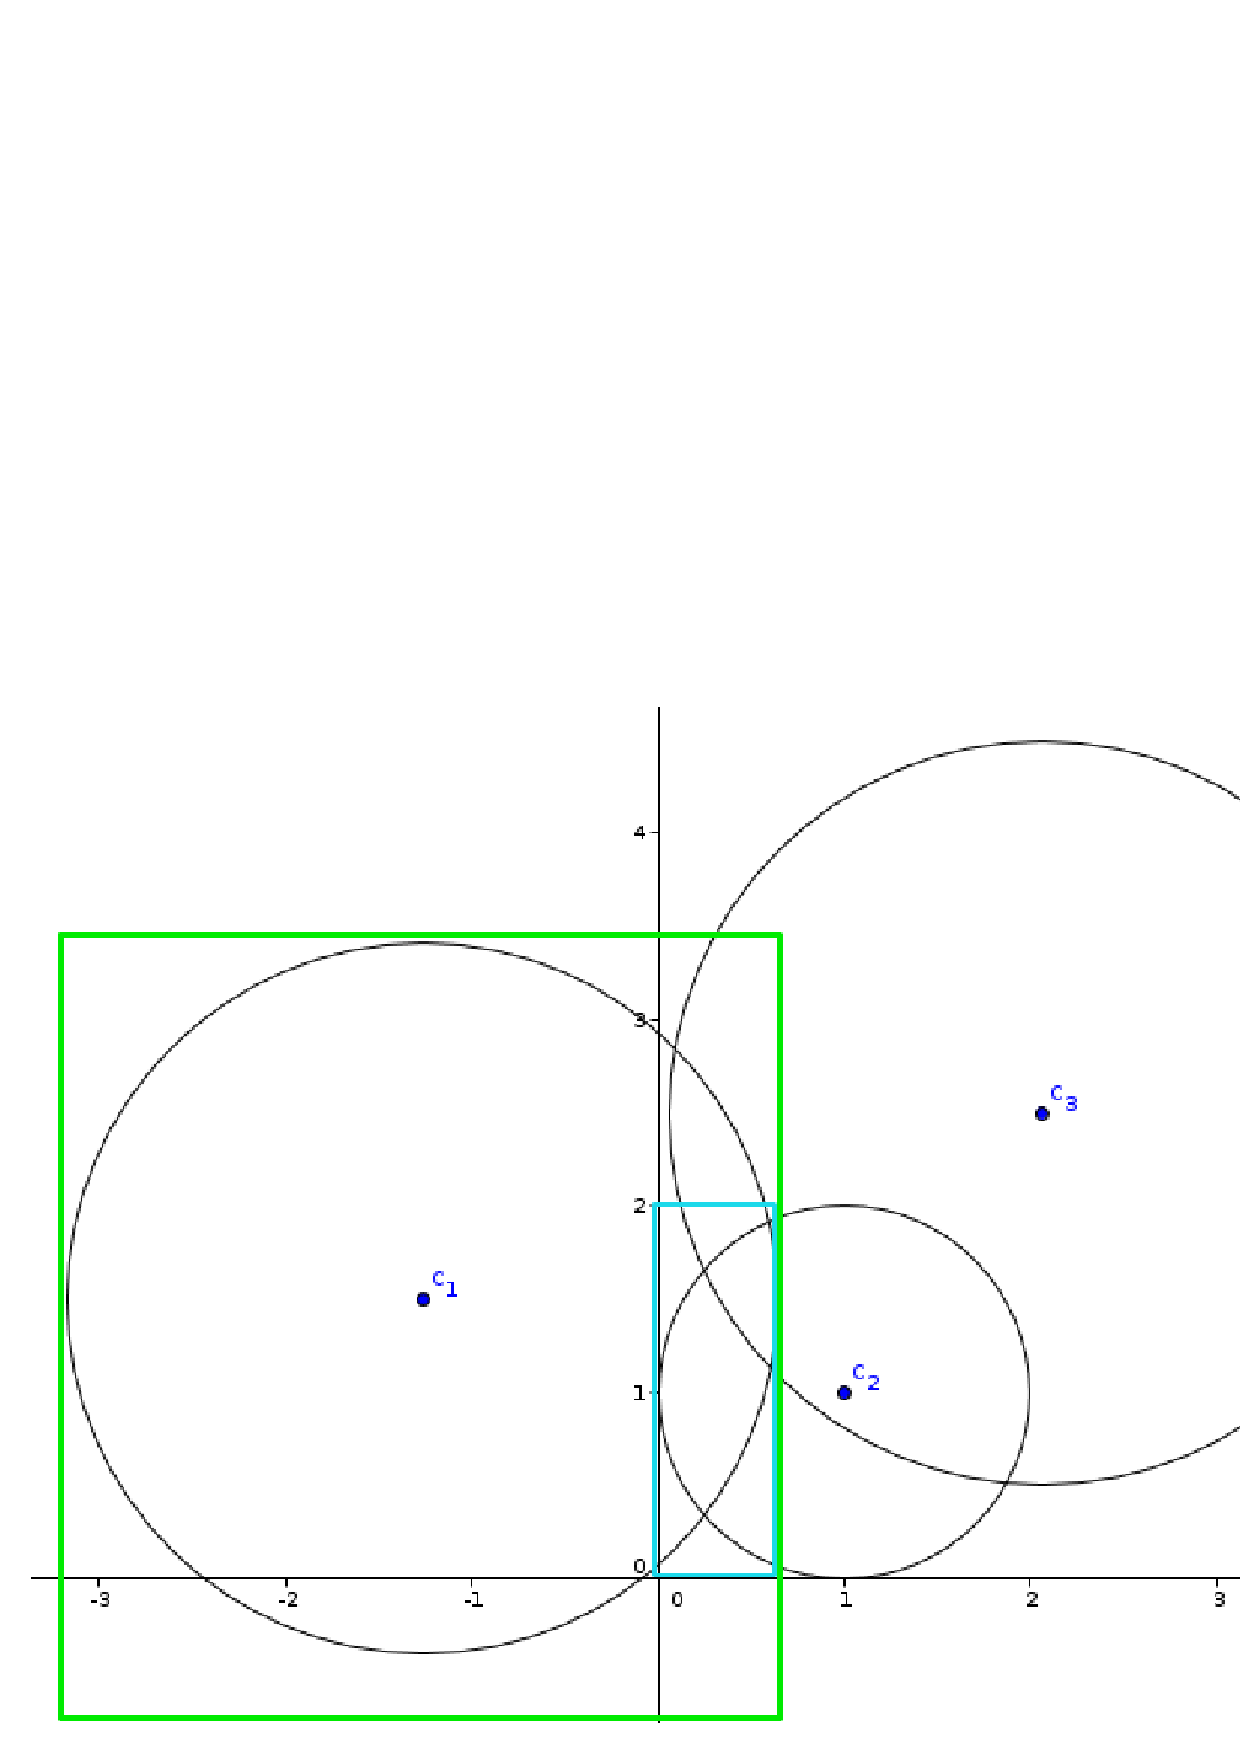
\includegraphics[width=0.55\textwidth]{img/hull2}
        \end{center}
      \end{figure}
   \begin{equation*}
       (x-x_{c_2})²+(y-y_{c_2})² = r_{c_2}²
    \end{equation*}
    }
    \onlySlide*{4}{
    \emph{Hull-consistance} : 3\up{ère} étape
      \begin{figure}[t]
        \begin{center}
          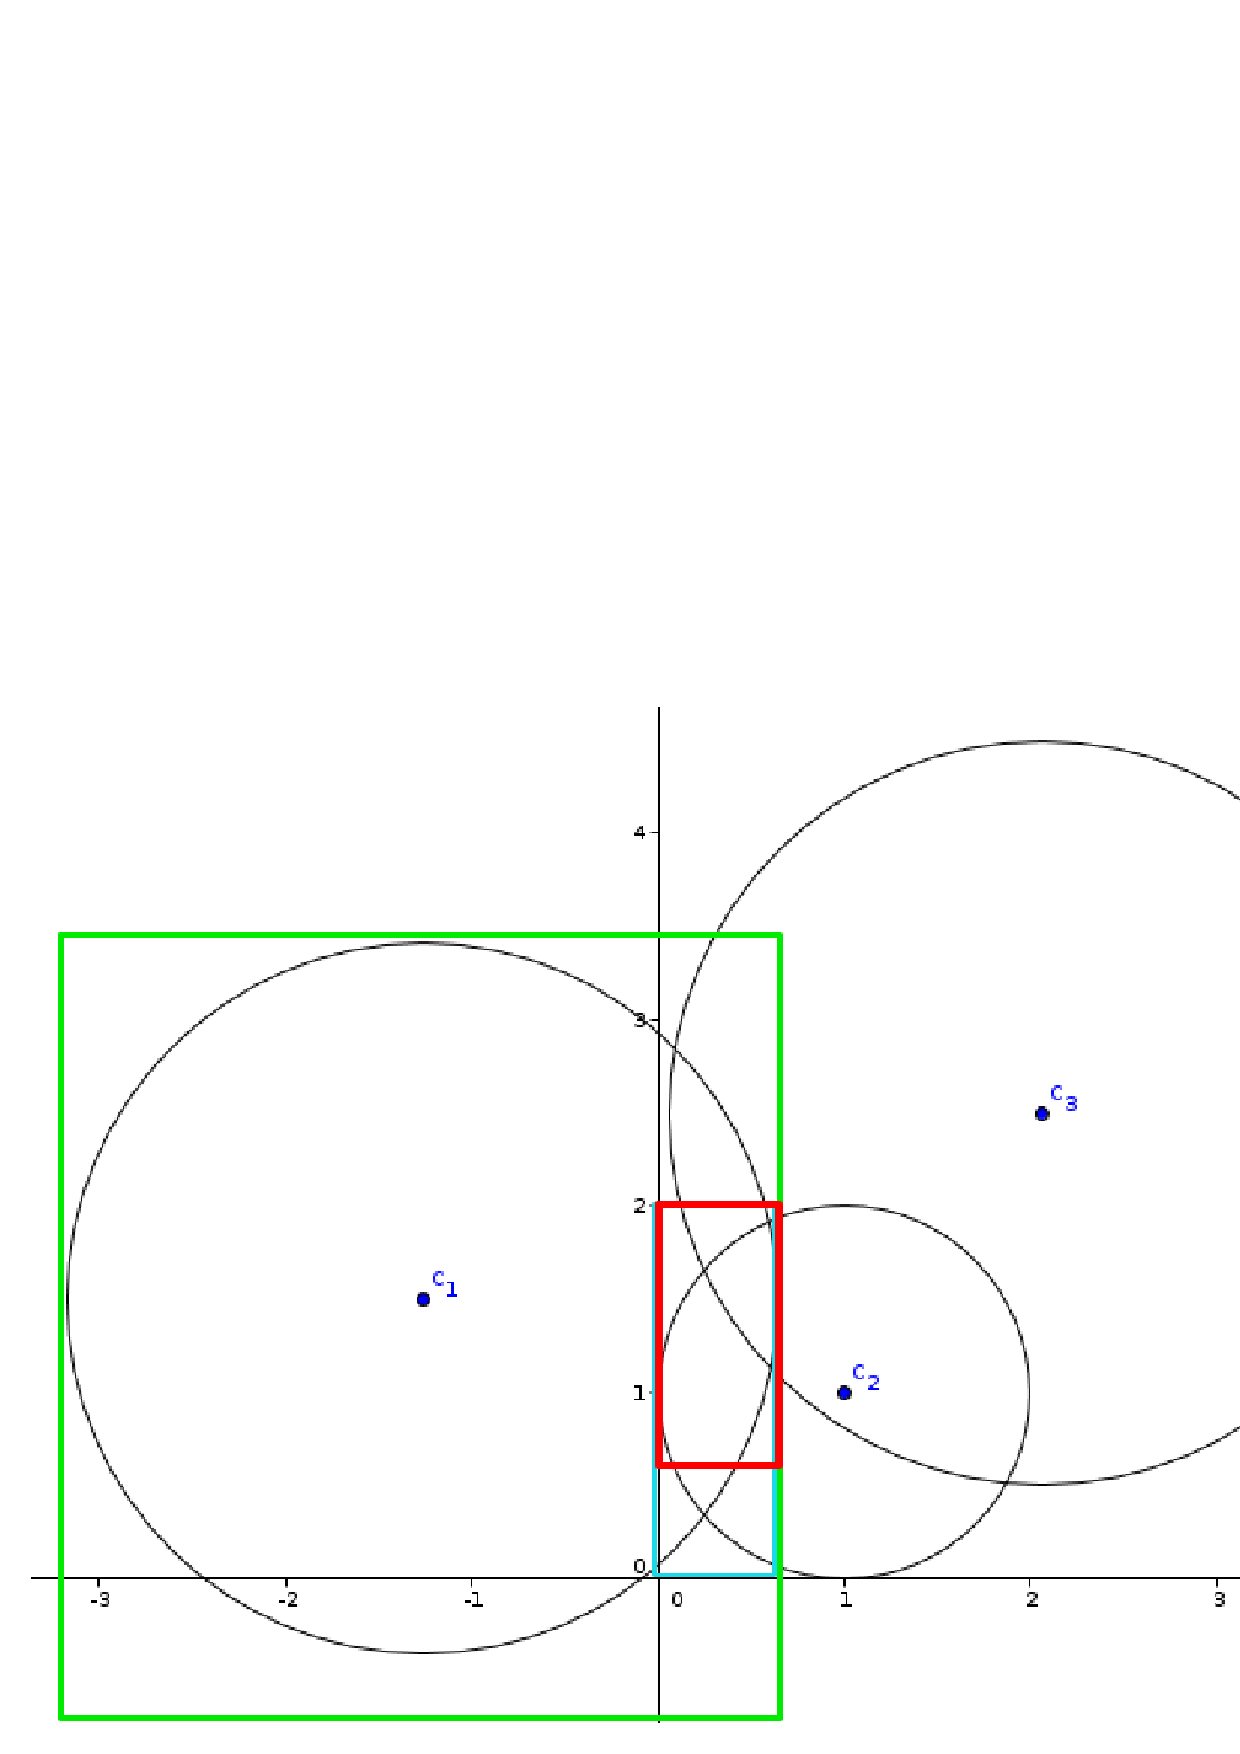
\includegraphics[width=0.55\textwidth]{img/hull3}
        \end{center}
      \end{figure}
    \begin{equation*}
        (x-x_{c_3})²+(y-y_{c_3})² = r_{c_3}²
    \end{equation*}
    }
  \end{slide}
}
 
%%%%%%%%%%%%%%%%%%%%%%%%%%%%%%%%%%%%%%%%%%%%%%%%%%%%%%%%%%%%%%%%%%%%%%%%%%%%
\overlays{3}{
  \begin{slide}[Box]{Exemple de \emph{Branch and Prune} :\\  Intersection de deux cercles}
    \slidetextsize
    \onlySlide*{1}{1\up{ère} Étape : \emph{Pruning}
      \begin{figure}[t]
        \begin{center}
          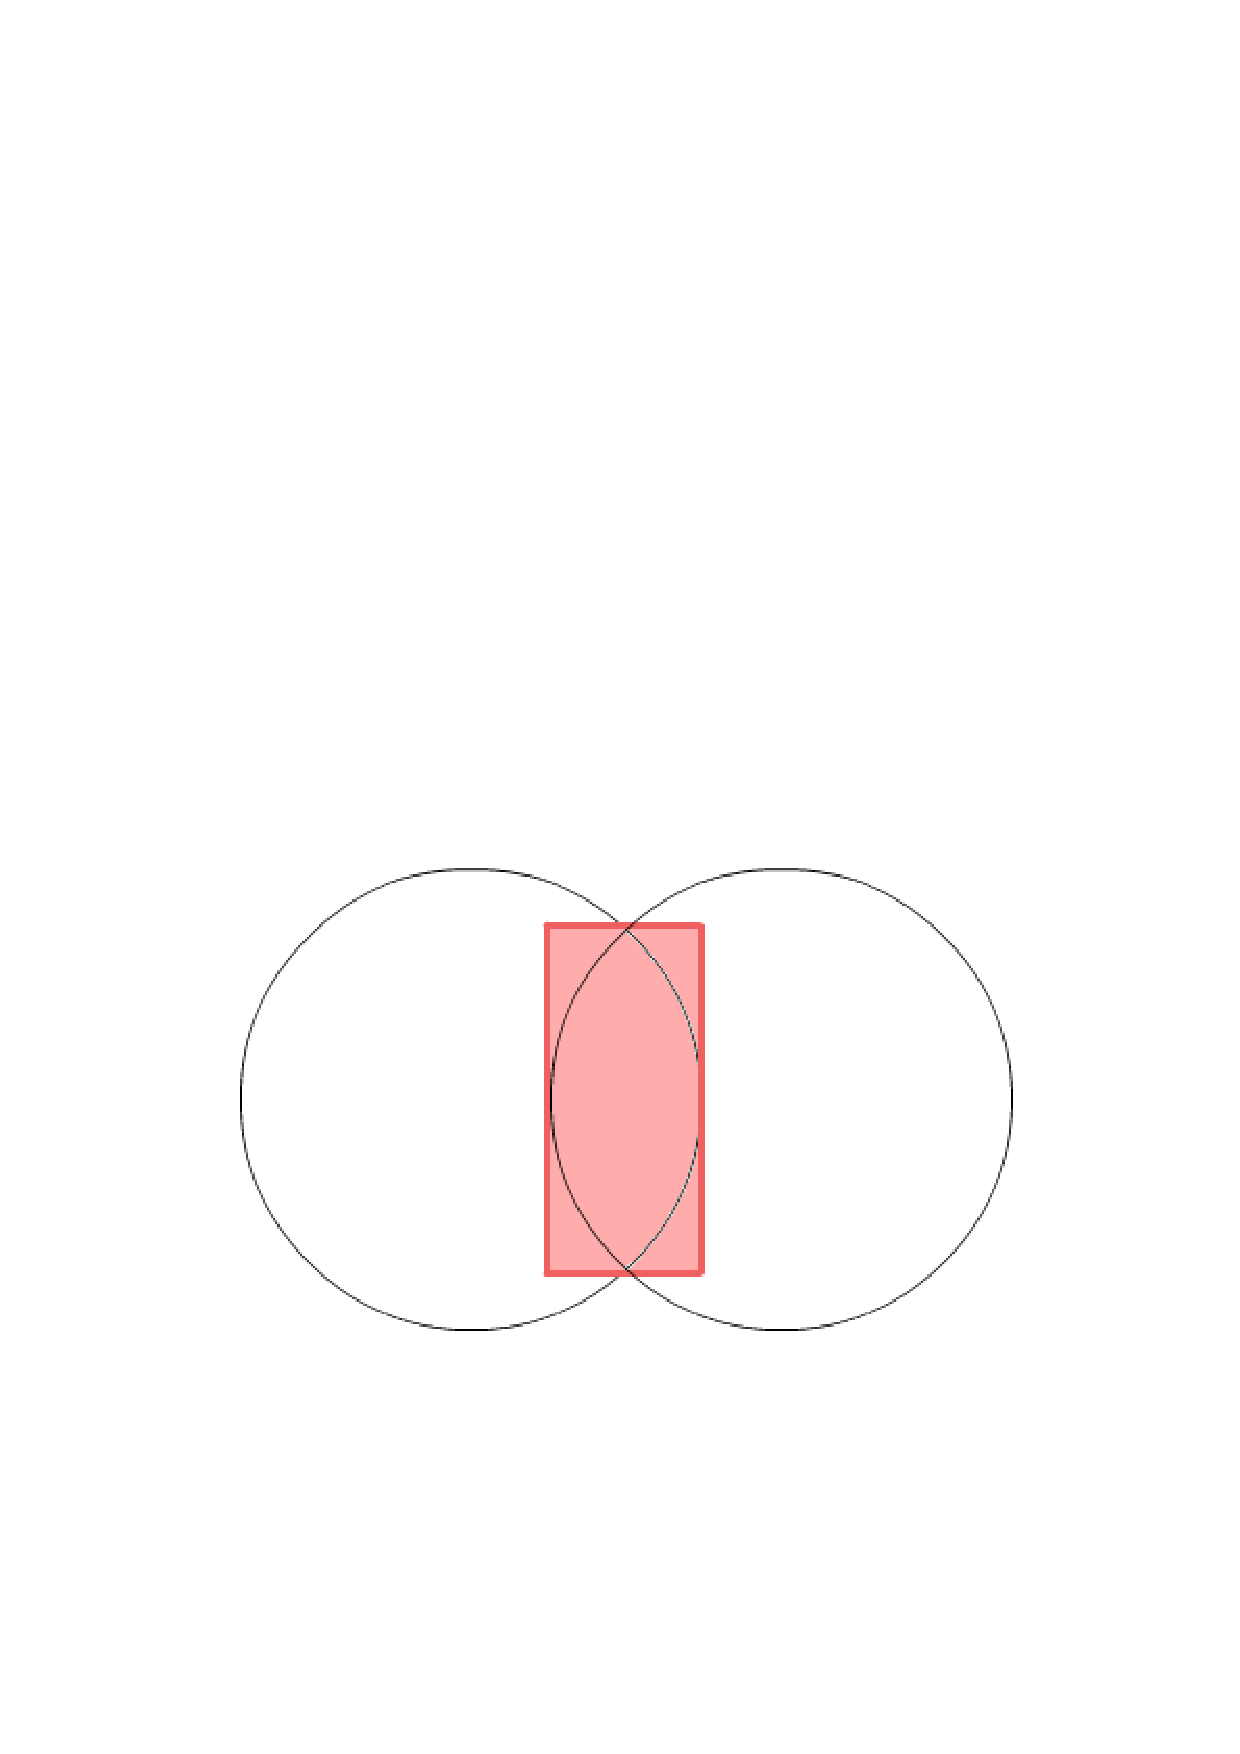
\includegraphics[width=0.65\textwidth]{img/BP}
        \end{center}
      \end{figure}
    }      
    \onlySlide*{2}{2\up{nd} Étape : \emph{Branch}
      \begin{figure}[t]
        \begin{center}
          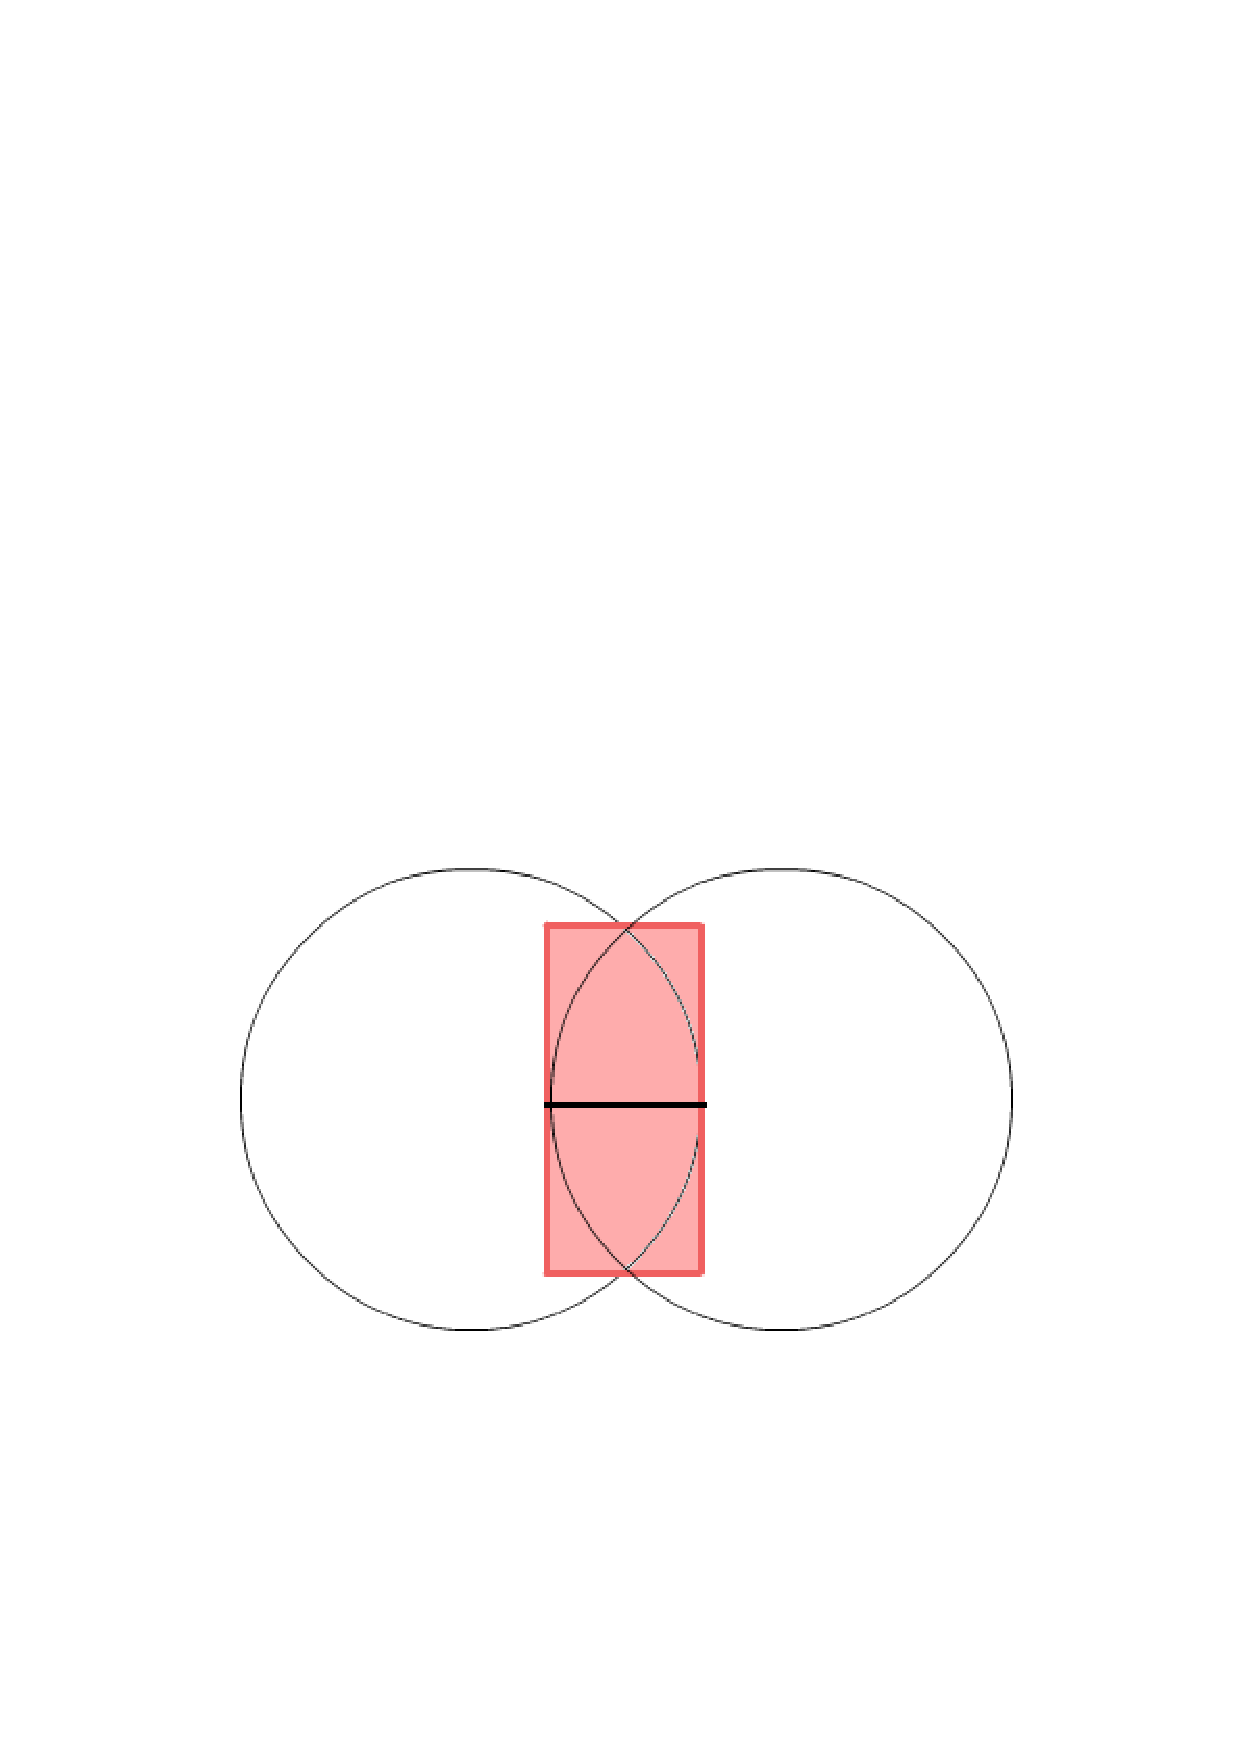
\includegraphics[width=0.65\textwidth]{img/BP2}
        \end{center}
      \end{figure}
    }
    \fromSlide{3}{3\up{ème} Étape :\emph{Pruning}
      \begin{figure}[t]
        \begin{center}
          
          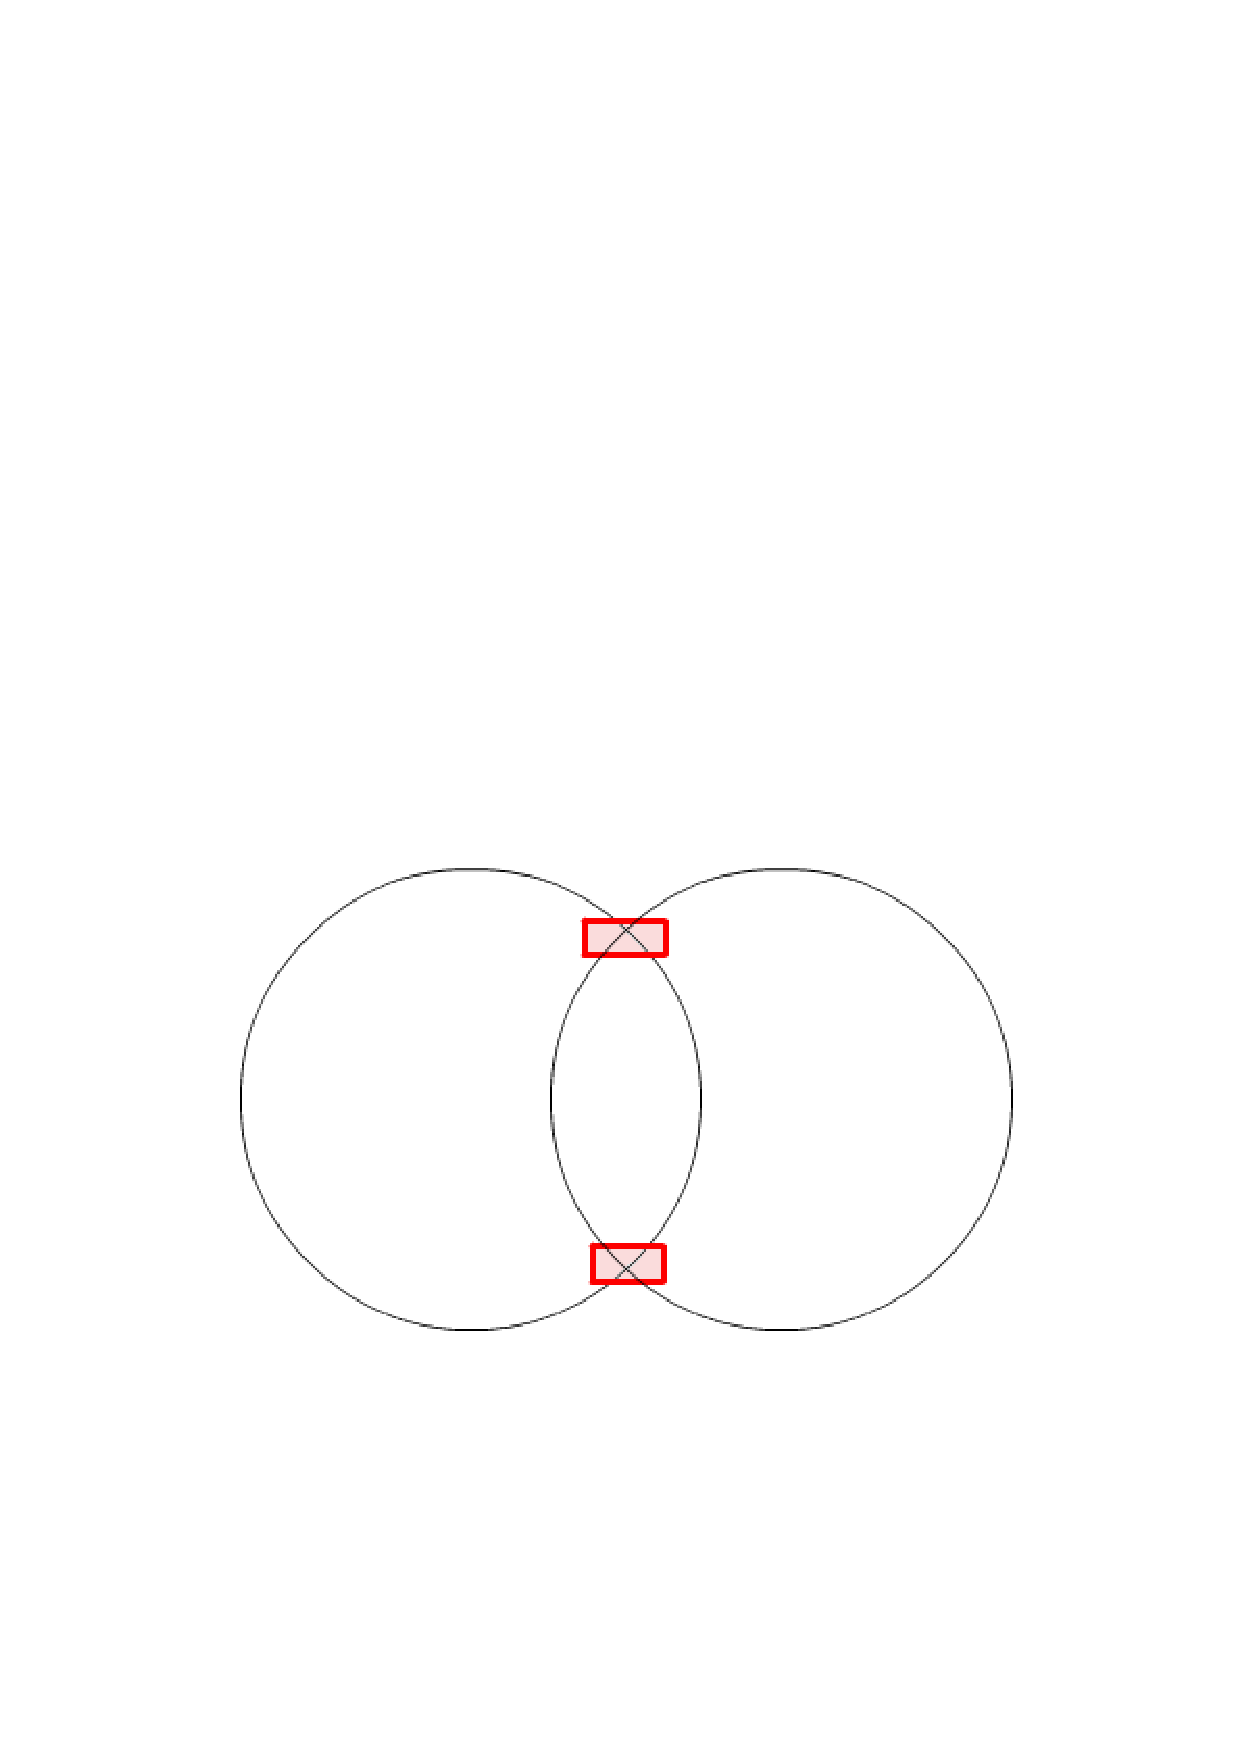
\includegraphics[width=0.65\textwidth]{img/BP3}
        \end{center}
      \end{figure}
    }

\end{slide}}

 %% %%%%%%%%%%%%%%%%%%%%%%%%%%%%%%%%%%%%%%%%%%%%%%%%%%%%%%%%%%%%%%%%%%%%%%%%%%%%%  
  \begin{slide}[Box]{Realpaver : présentation}
    \slidetextsize
    Méthodes de résolutions de contraintes géométriques par propagation d’intervalles.
    \begin{figure}[t]\centering \includegraphics[width=0.35\textwidth]{img/disk-disk.ps}\end{figure}
  \end{slide}
 %% %%%%%%%%%%%%%%%%%%%%%%%%%%%%%%%%%%%%%%%%%%%%%%%%%%%%%%%%%%%%%%%%%%%%%%%%%%%%%  
\begin{slide}{Realpaver : exemple de modèle}
\hypertarget{code}{ }
\tiny\vspace{-.35in}\hspace{-.35in}
\begin{verbatim}
Constants
x0 = -1,
y0 = 0,
R0 = 2,
x1 = 1,
y1 = 0,
R1 = 2
;
Variables
x in ]-oo,
y in ]-oo,
;
Constraints
(x-x0)^2 +
(x-x1)^2 +
;
+oo[,
+oo[
(y-y0)^2 <= R0^2,
(y-y1)^2 <= R1^2
\end{verbatim}
\end{slide}
 %%%%%%%%%%%%%%%%%%%%%%%%%%%%%%%%%%%%%%%%%%%%%%%%%%%%%%%%%%%%%%%%%%%%%%%%%%%% 
\begin{slide}{Realpaver : exemple de sortie}
\hypertarget{code}{ }
\tiny\vspace{-.35in}
\begin{verbatim}
RealPaver v. 0.4 (c) LINA 2004
INITIAL BOX
x in ]-oo , +oo[
y in ]-oo , +oo[
OUTER BOX 1
x in [0.7924334198270921 , 0.795689483022687]
y in [0.8806243697296342 , 0.8872330220900007]
...
OUTER BOX 3053
x in [-0.7956894830226868 , -0.7924334198270919]
y in [-0.8872330220900011 , -0.8806243697296345]
precision: 0.00661, elapsed time: 150 ms
END OF SOLVING
Property: reliable process (no solution is lost)
Elapsed time: 150 ms
\end{verbatim}
\end{slide}
 %%%%%%%%%%%%%%%%%%%%%%%%%%%%%%%%%%%%%%%%%%%%%%%%%%%%%%%%%%%%%%%%%%%%%%%%%%%% 
\overlays{4}{
  \begin{slide}[Box]{Définition d'une boîte}
       \slidetextsize
    \textbf{Entité atomique du pavage}
    \begin{Itemize}
      \fromSlide{2}{\item Un identifiant 
        \begin{Itemize}
        \item NUMBER
        \item STRING
        \end{Itemize}}
      \fromSlide{3}{\item Une liste de coordonnées
        \begin{Itemize}
        \item INTERVAL
      \end{Itemize}}
      \fromSlide{4}{\item Une liste des caractéristiques
        \begin{Itemize}
        \item NUMBER
        \item STRING
        \item INTERVAL
      \end{Itemize}}
    \end{Itemize}
  \end{slide}
}
%% %%%%%%%%%%%%%%%%%%%%%%%%%%%%%%%%%%%%%%%%%%%%%%%%%%%%%%%%%%%%%%%%%%%%%%%%%%%%
\overlays{4}{
  \begin{slide}[Box]{Étude des structures de données pour une boîte}
    \textbf{Structure de données}
    \begin{Itemize}
      \fromSlide{2}{\item Un tableau}
      \fromSlide{3}{\item Une liste}
      \fromSlide{4}{\item Une table de hachage}
    \end{Itemize}
  \end{slide}
}
%%%%%%%%%%%%%%%%%%%%%%%%%%%%%%%%%%%%%%%%%%%%%%%%%%%%%%%%%%%%%%%%%%%%%%%%%%%%
  \begin{slide}[Box]{Étude des structures de données pour une boîte}
    \textbf{Tests expérimentaux}
    \begin{table}[h]
      \centering
      \begin{tabular}{|c|c|c|c|}
        \hline
        \backslashbox{Structure} {Nombre d'accès} & $10^6$ & $10^7$ & $10^8$ \\
        \hline
       3 HashMap & 0.31s& 2.86s & 28.56s\\
       \hline
       3 ArrayList & 0.20s & 1.81s & 17.49s\\
        \hline
       1 ArrayList & 0.19s & 1.58s & 15.12s\\
        \hline
       1 LinkedList & 0.31s & 2,79s &  27.59s\\
        \hline
      \end{tabular}
    \end{table}
    Relevé des temps CPU d'accès au caractéristiques en secondes
  \end{slide}
%%%%%%%%%%%%%%%%%%%%%%%%%%%%%%%%%%%%%%%%%%%%%%%%%%%%%%%%%%%%%%%%%%%%%%%%%%%%
\overlays{5}{
  \begin{slide}[Box]{Étude des structures de données pour un pavage}
    \textbf{Structure de données}
    \begin{Itemize}
      \fromSlide{2}{\item Vector}
      \fromSlide{3}{\item Dictionnaire}
      \fromSlide{4}{\item Arbre binaire}
      \fromSlide{5}{\item Arbre a-b}
    \end{Itemize}
  \end{slide}
}
%%%%%%%%%%%%%%%%%%%%%%%%%%%%%%%%%%%%%%%%%%%%%%%%%%%%%%%%%%%%%%%%%%%%%%%%%%%%
  \begin{slide}[Box]{Visualisation : QuadTree}
    \textbf{Exemple de représentation}
      \begin{figure}[t]
        \begin{center}
          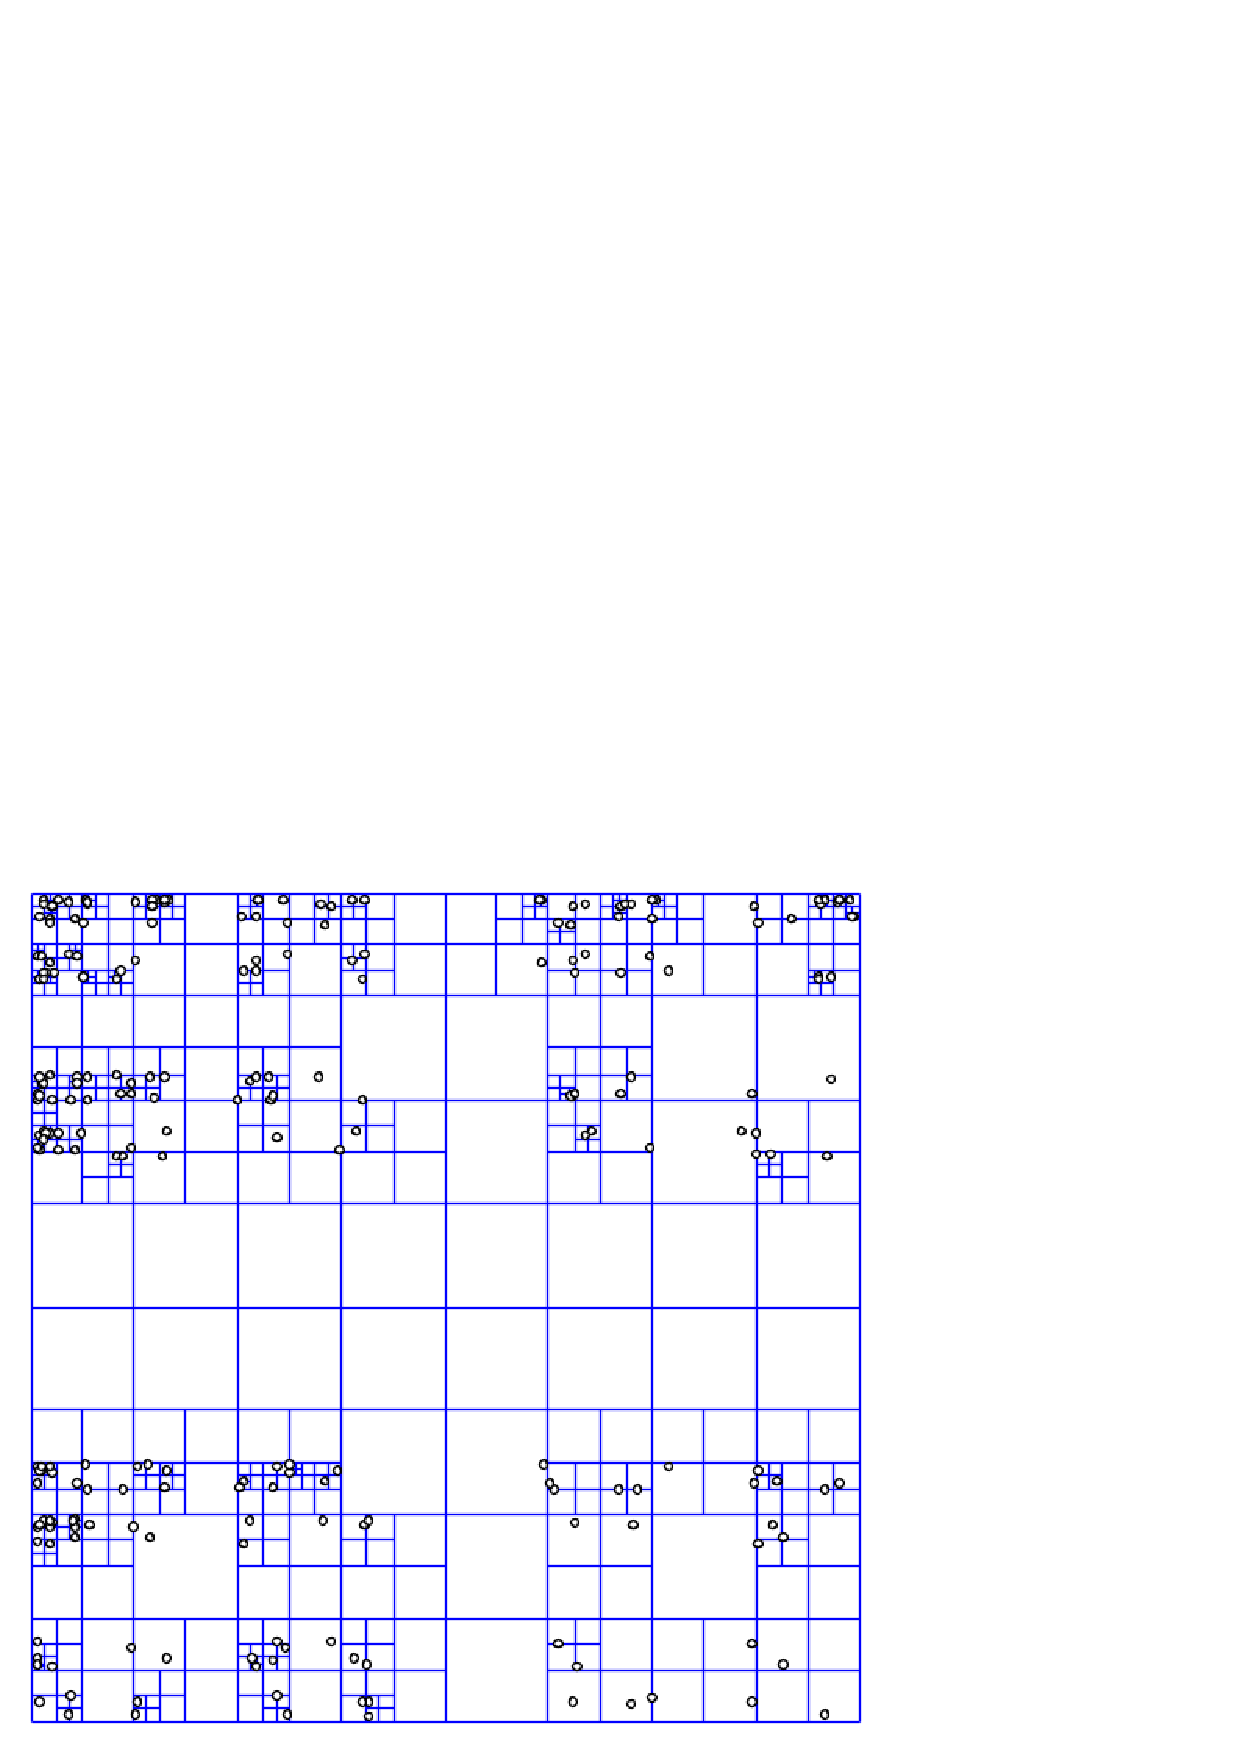
\includegraphics[width=0.55\textwidth]{img/quadtree}
        \end{center}
      \end{figure}
  \end{slide}
%% %%%%%%%%%%%%%%%%%%%%%%%%%%%%%%%%%%%%%%%%%%%%%%%%%%%%%%%%%%%%%%%%%%%%%%%%%%%%
  \begin{slide}[Box]{Visualisation : QuadTree}
    %    \slidetextsiz
    \textbf{Algorithme}
    \begin{table}[htbp]
      \centering
      \begin{tabular}{|c|cccc|}
        \hline
   Cas de récursion & 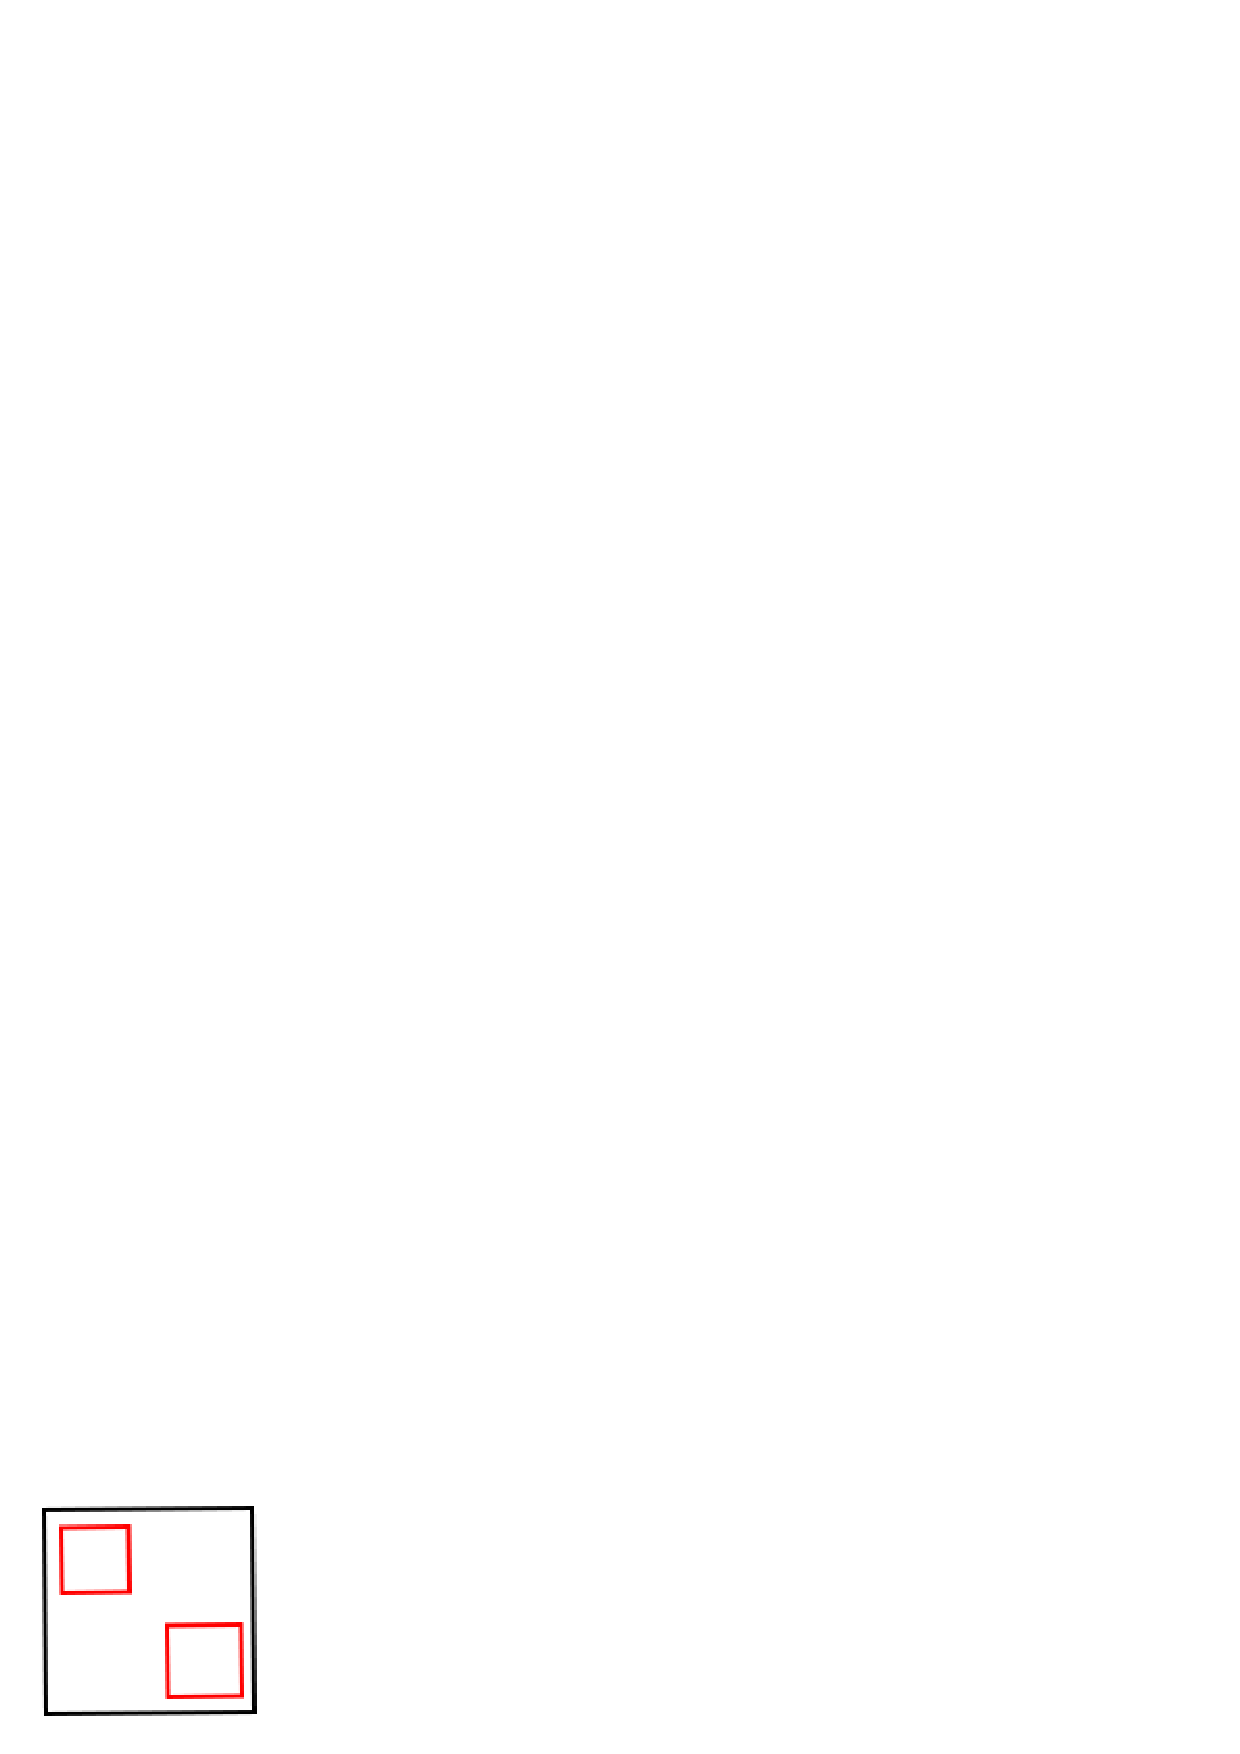
\includegraphics[scale=0.20]{img/QT4}&  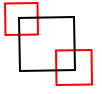
\includegraphics[scale=0.20]{img/QT5}& &\\
   \hline
   Cas d'arrêt&  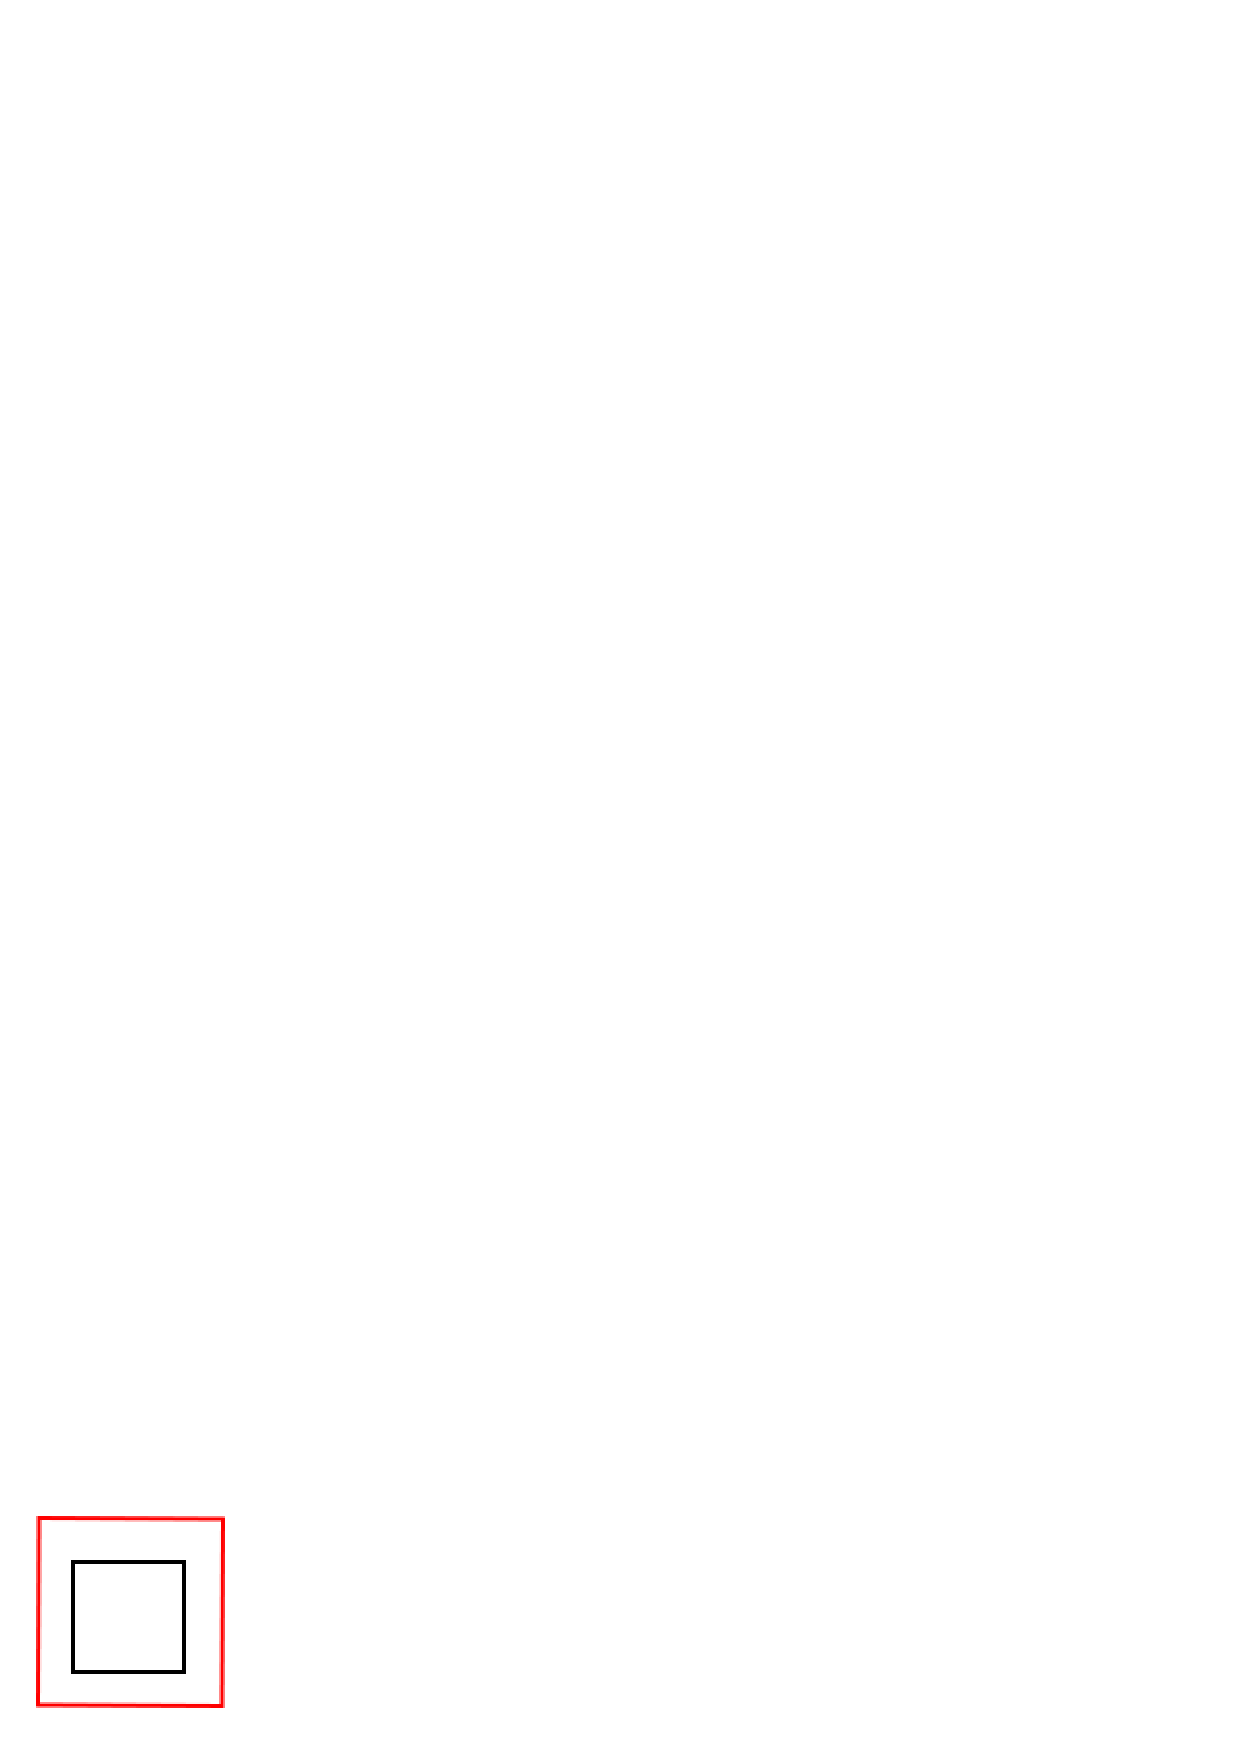
\includegraphics[scale=0.20]{img/QT1}&  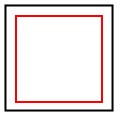
\includegraphics[scale=0.20]{img/QT2}&  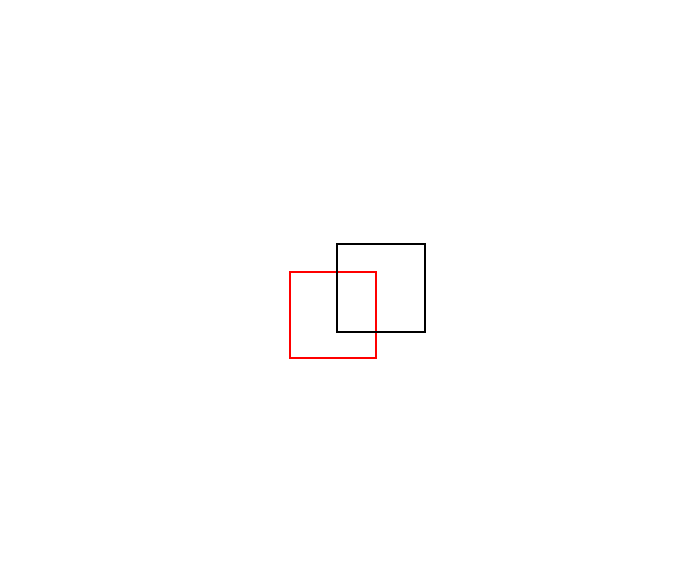
\includegraphics[scale=0.20]{img/QT3}&  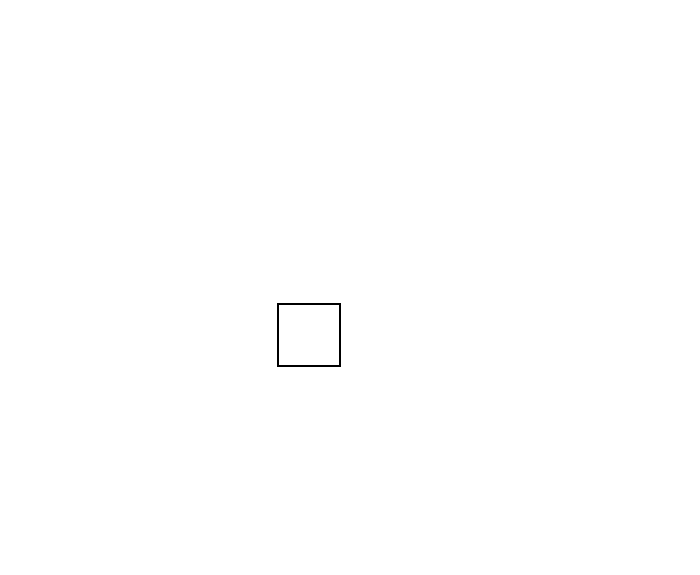
\includegraphics[scale=0.30]{img/QT6}\\
   \hline
      \end{tabular}
    \end{table}
Classification visuelle des cas d'arrêts et de récursions

  \end{slide}
  %% %%%%%%%%%%%%%%%%%%%%%%%%%%%%%%%%%%%%%%%%%%%%%%%%%%%%%%%%%%%%%%%%%%%%%%%%%%%%
\overlays{3}{
  \begin{slide}[Box]{Visualisation : QuadTree}
    %    \slidetextsiz
    \textbf{Inconvénients du QuadTree}
    \begin{Itemize}
      \fromSlide{2}{\item Structure peu adaptée pour stocker des éléments de dimension $d$}
      \fromSlide{3}{\item Problèmes des \emph{frontières}}
    \end{Itemize}
  \end{slide}
}
  %%%%%%%%%%%%%%%%%%%%%%%%%%%%%%%%%%%%%%%%%%%%%%%%%%%%%%%%%%%%%%%%%%%%%%%%%%%%

  \begin{slide}[Box]{Visualisation : QuadTree}
      \textbf{Cas de superposition des boîtes}
      \begin{figure}[t]
        \begin{center}
          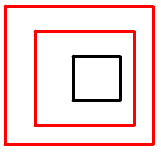
\includegraphics[width=0.25\textwidth]{img/QT8}
        \end{center}
      \end{figure}
  \end{slide}
  %%%%%%%%%%%%%%%%%%%%%%%%%%%%%%%%%%%%%%%%%%%%%%%%%%%%%%%%%%%%%%%%%%%%%%%%%%%%

\overlays{6}{
  \begin{slide}[Box]{Visualisation : QuadTree}
      \textbf{Le problème des \emph{frontières}}
   \onlySlide*{1}{
   \begin{figure}[t]
        \begin{center}
          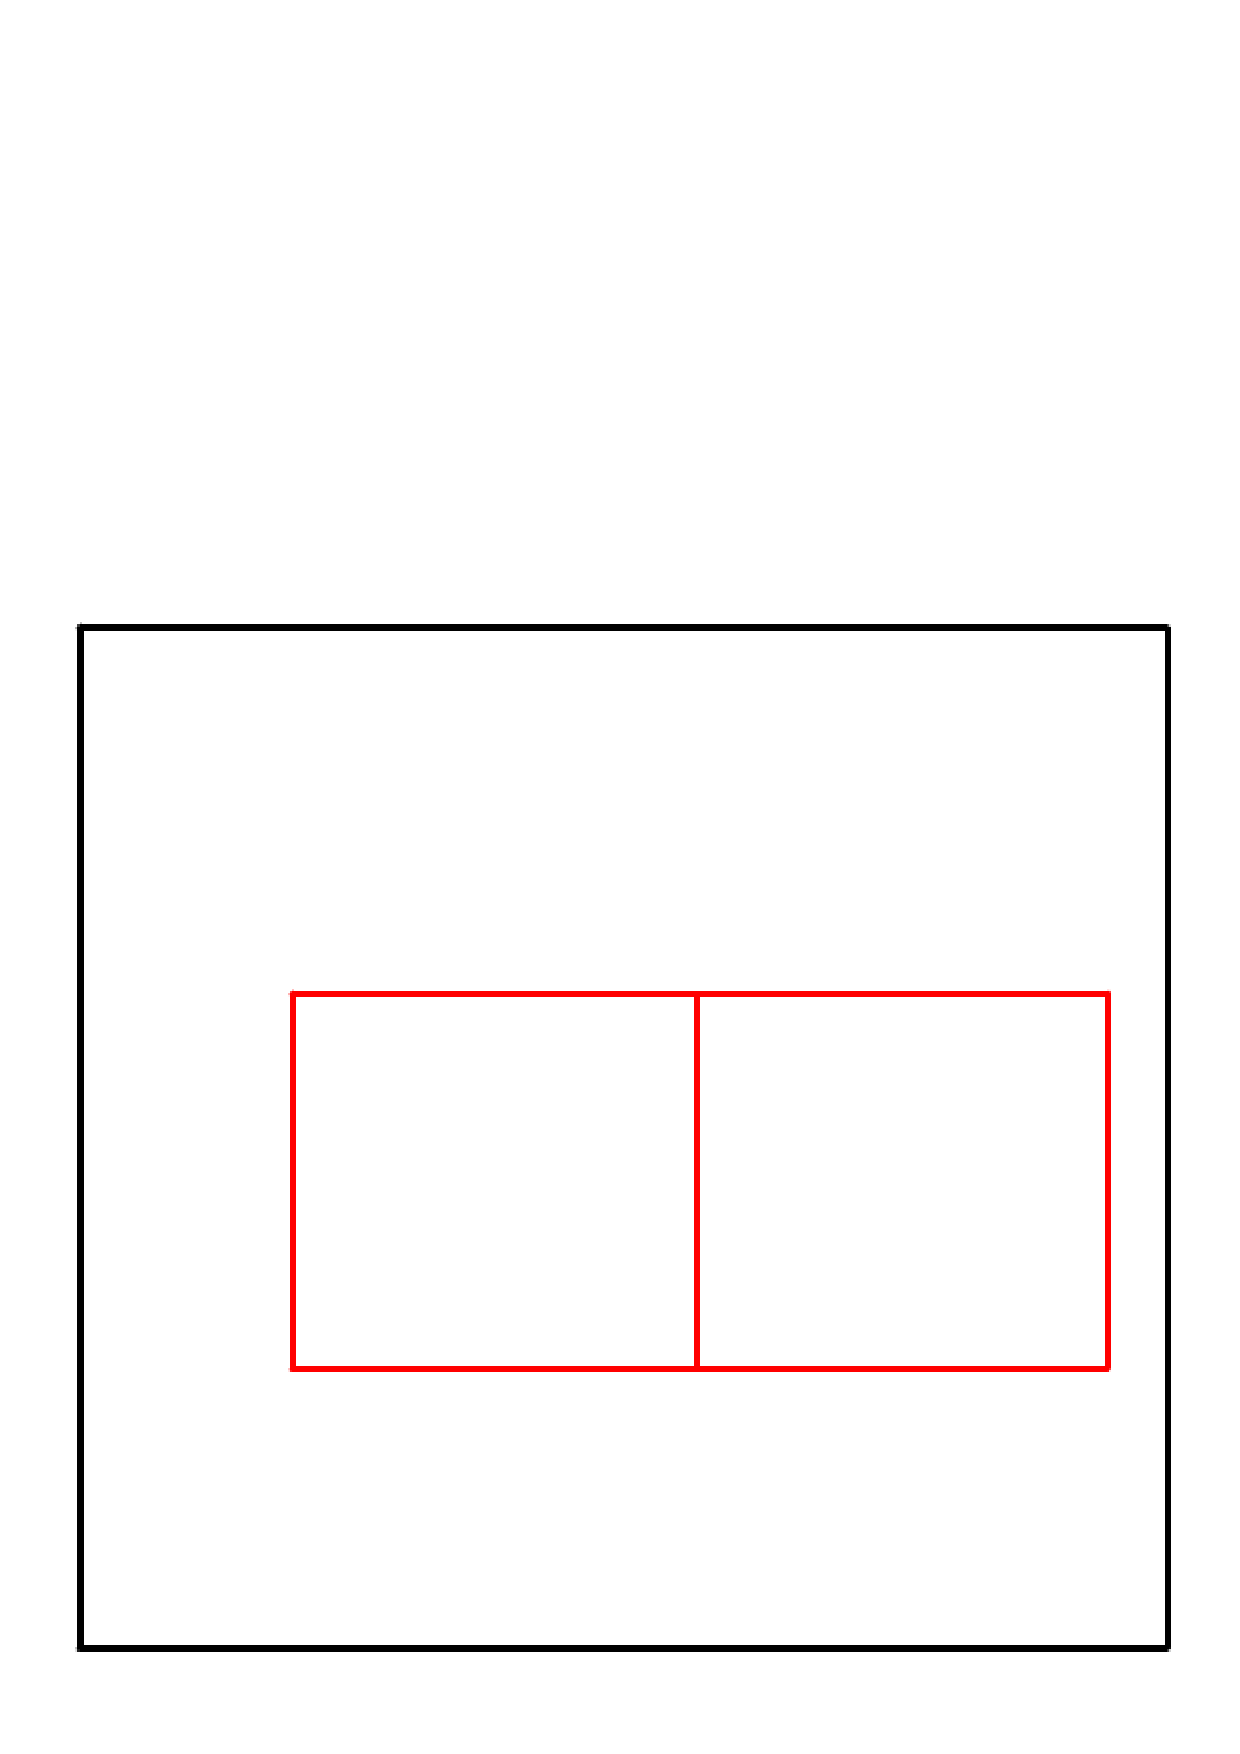
\includegraphics[width=0.50\textwidth]{img/SQT1}
        \end{center}
      \end{figure}
}
   \onlySlide*{2}{
   \begin{figure}[t]
        \begin{center}
          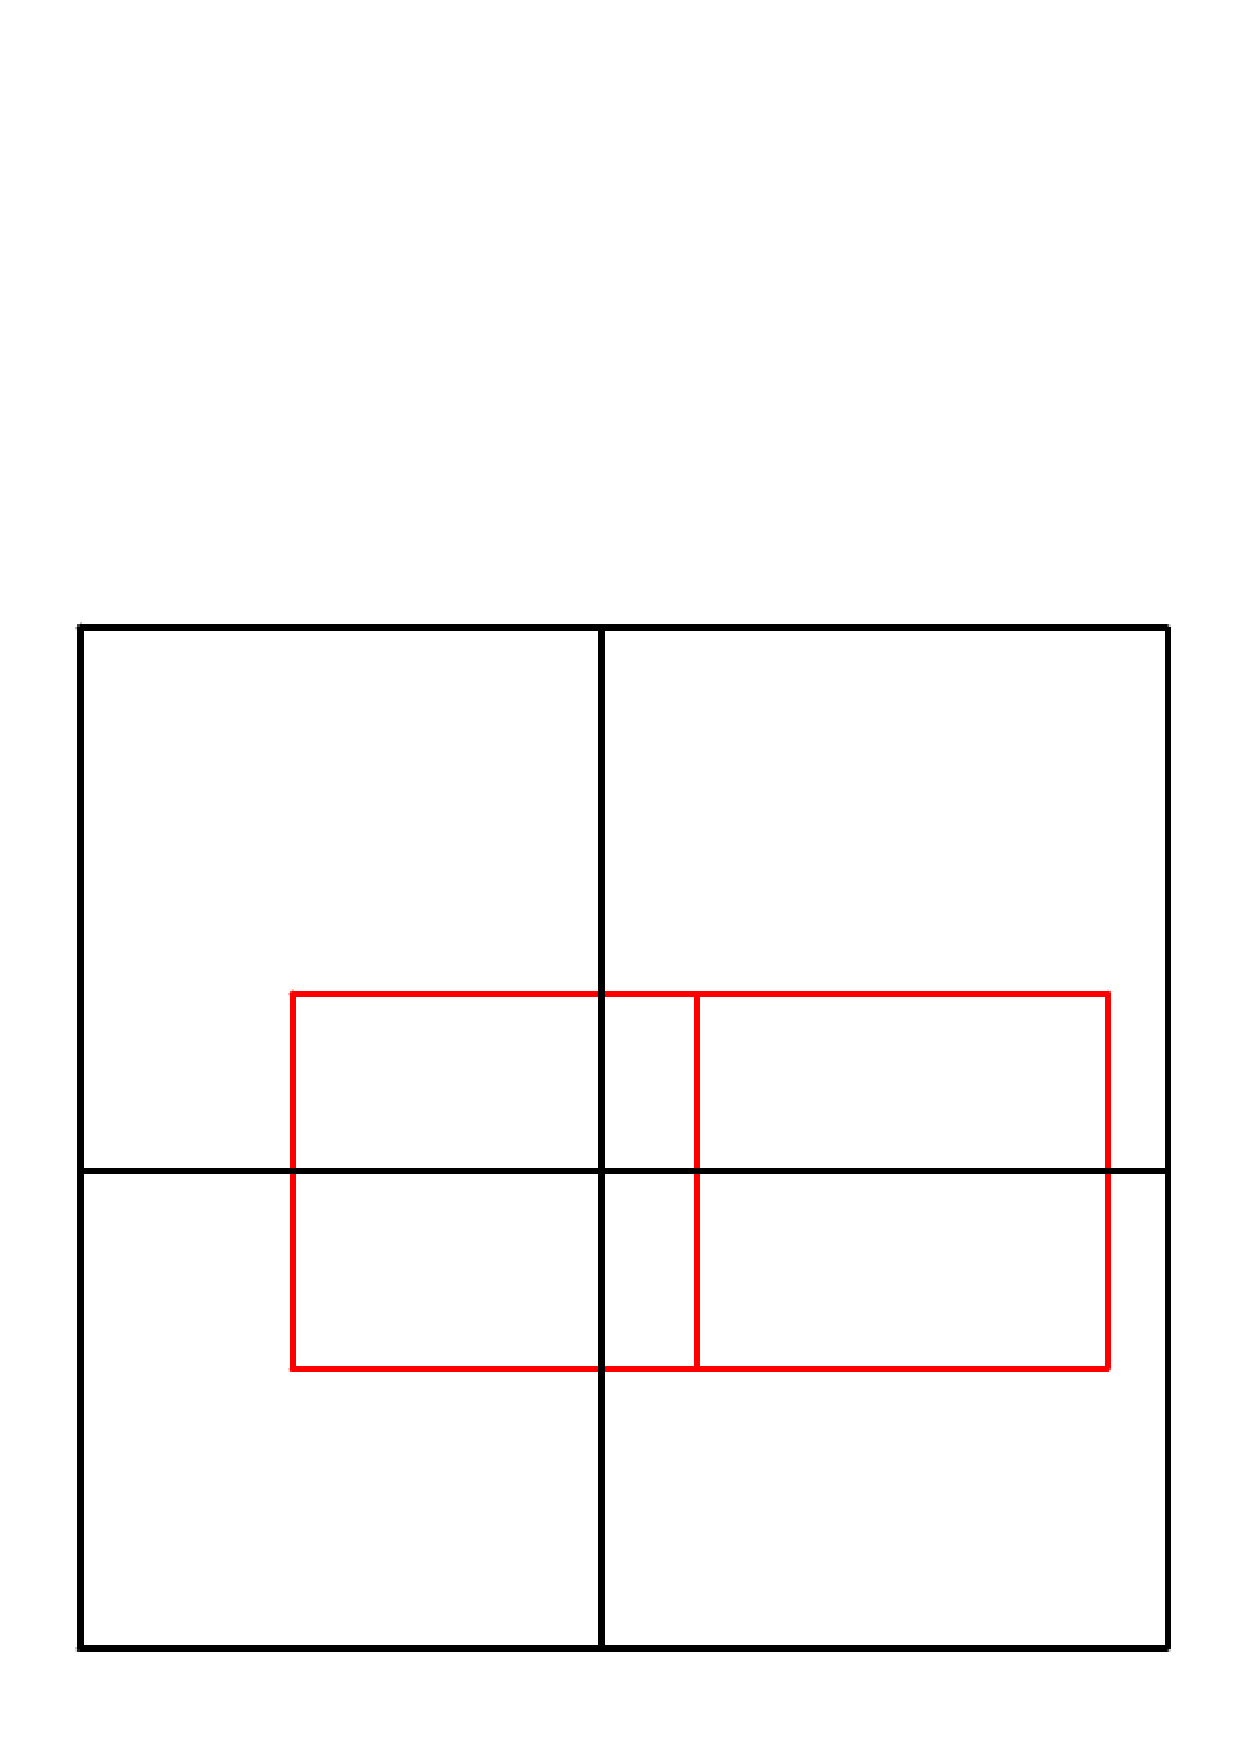
\includegraphics[width=0.50\textwidth]{img/SQT2}
        \end{center}
      \end{figure}
}
   \onlySlide*{3}{
     \begin{figure}[t]
       \begin{center}
         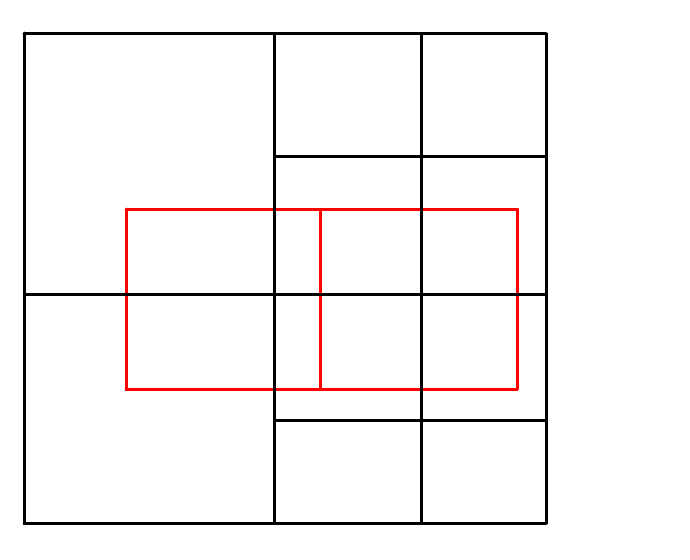
\includegraphics[width=0.50\textwidth]{img/SQT3}
       \end{center}
     \end{figure}
   }
   \onlySlide*{4}{
   \begin{figure}[t]
        \begin{center}
          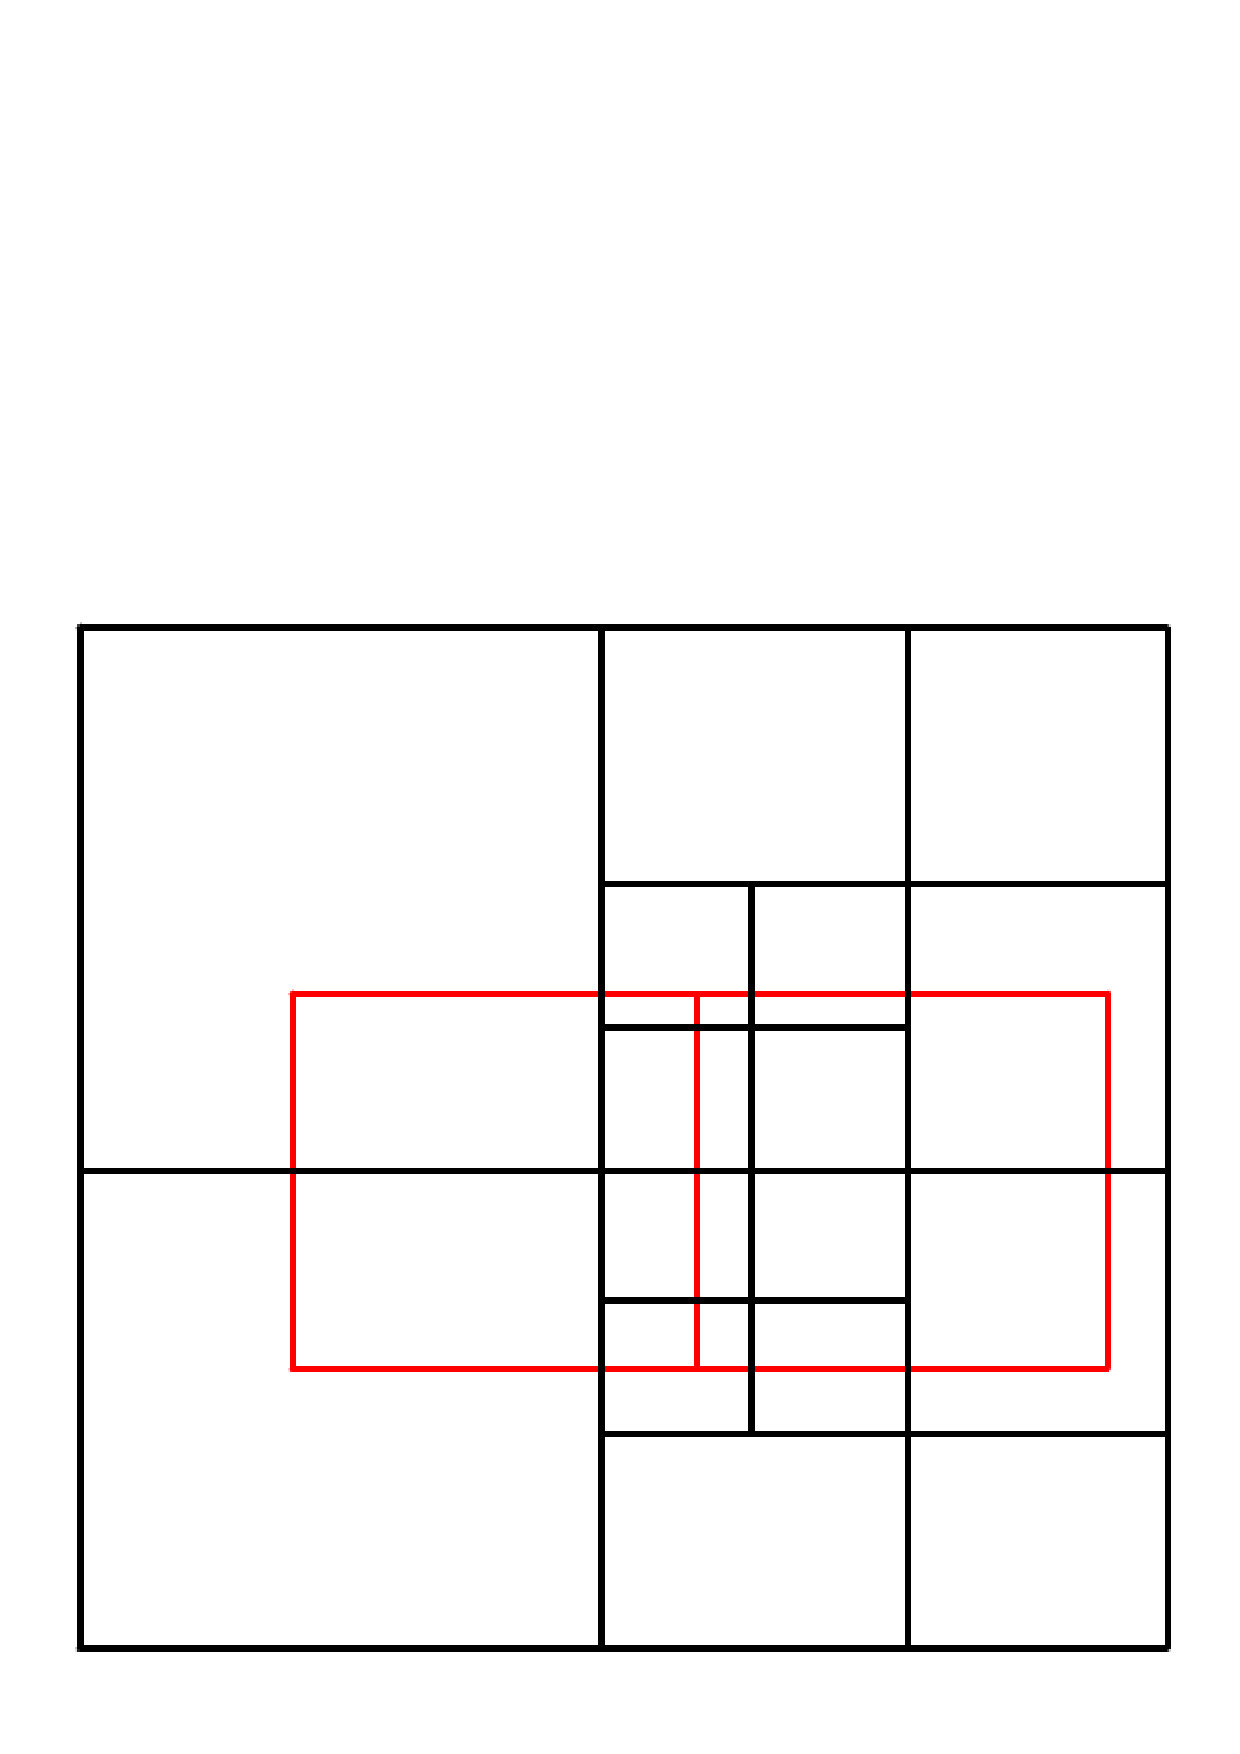
\includegraphics[width=0.50\textwidth]{img/SQT4}
        \end{center}
      \end{figure}
}
   \onlySlide*{5}{
   \begin{figure}[t]
        \begin{center}
          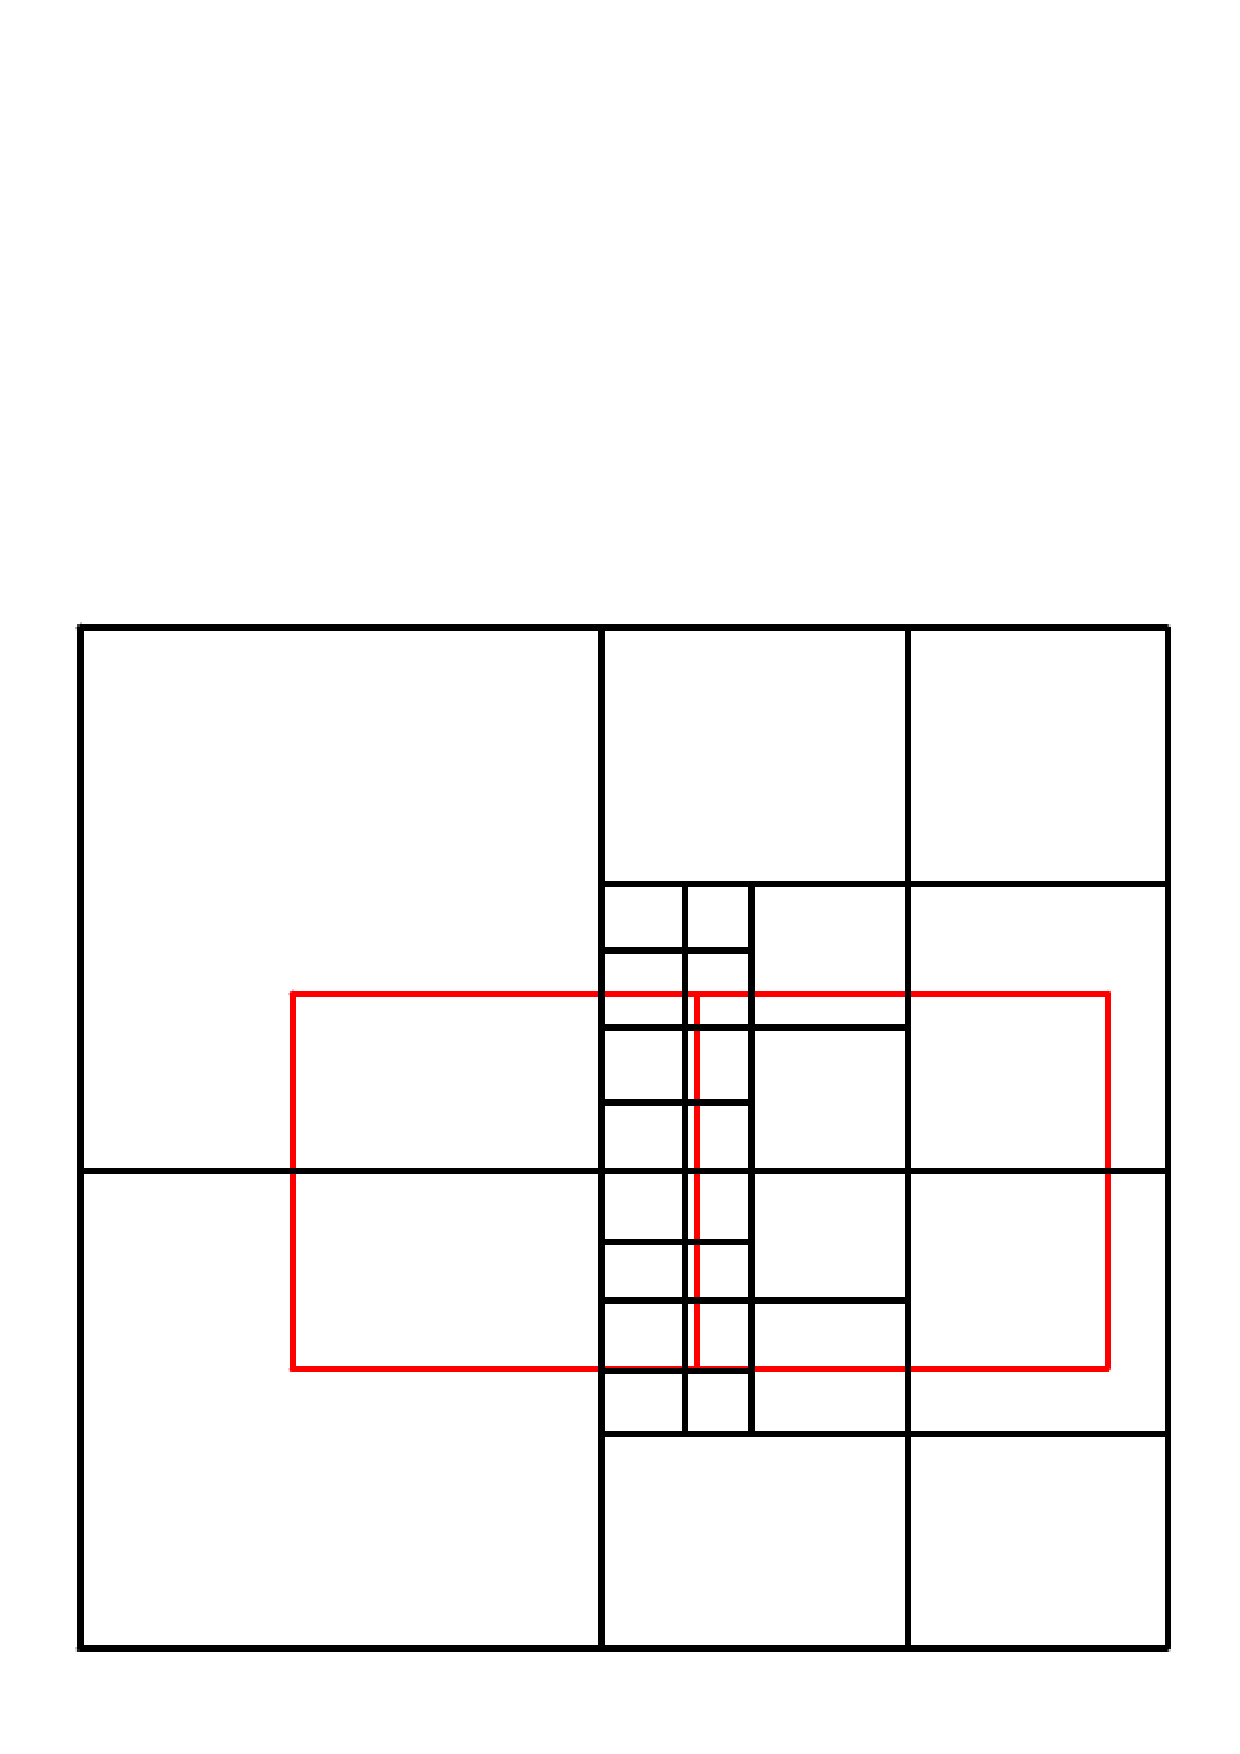
\includegraphics[width=0.50\textwidth]{img/SQT5}
        \end{center}
      \end{figure}
}
   \fromSlide{6}{
   \begin{figure}[t]
        \begin{center}
          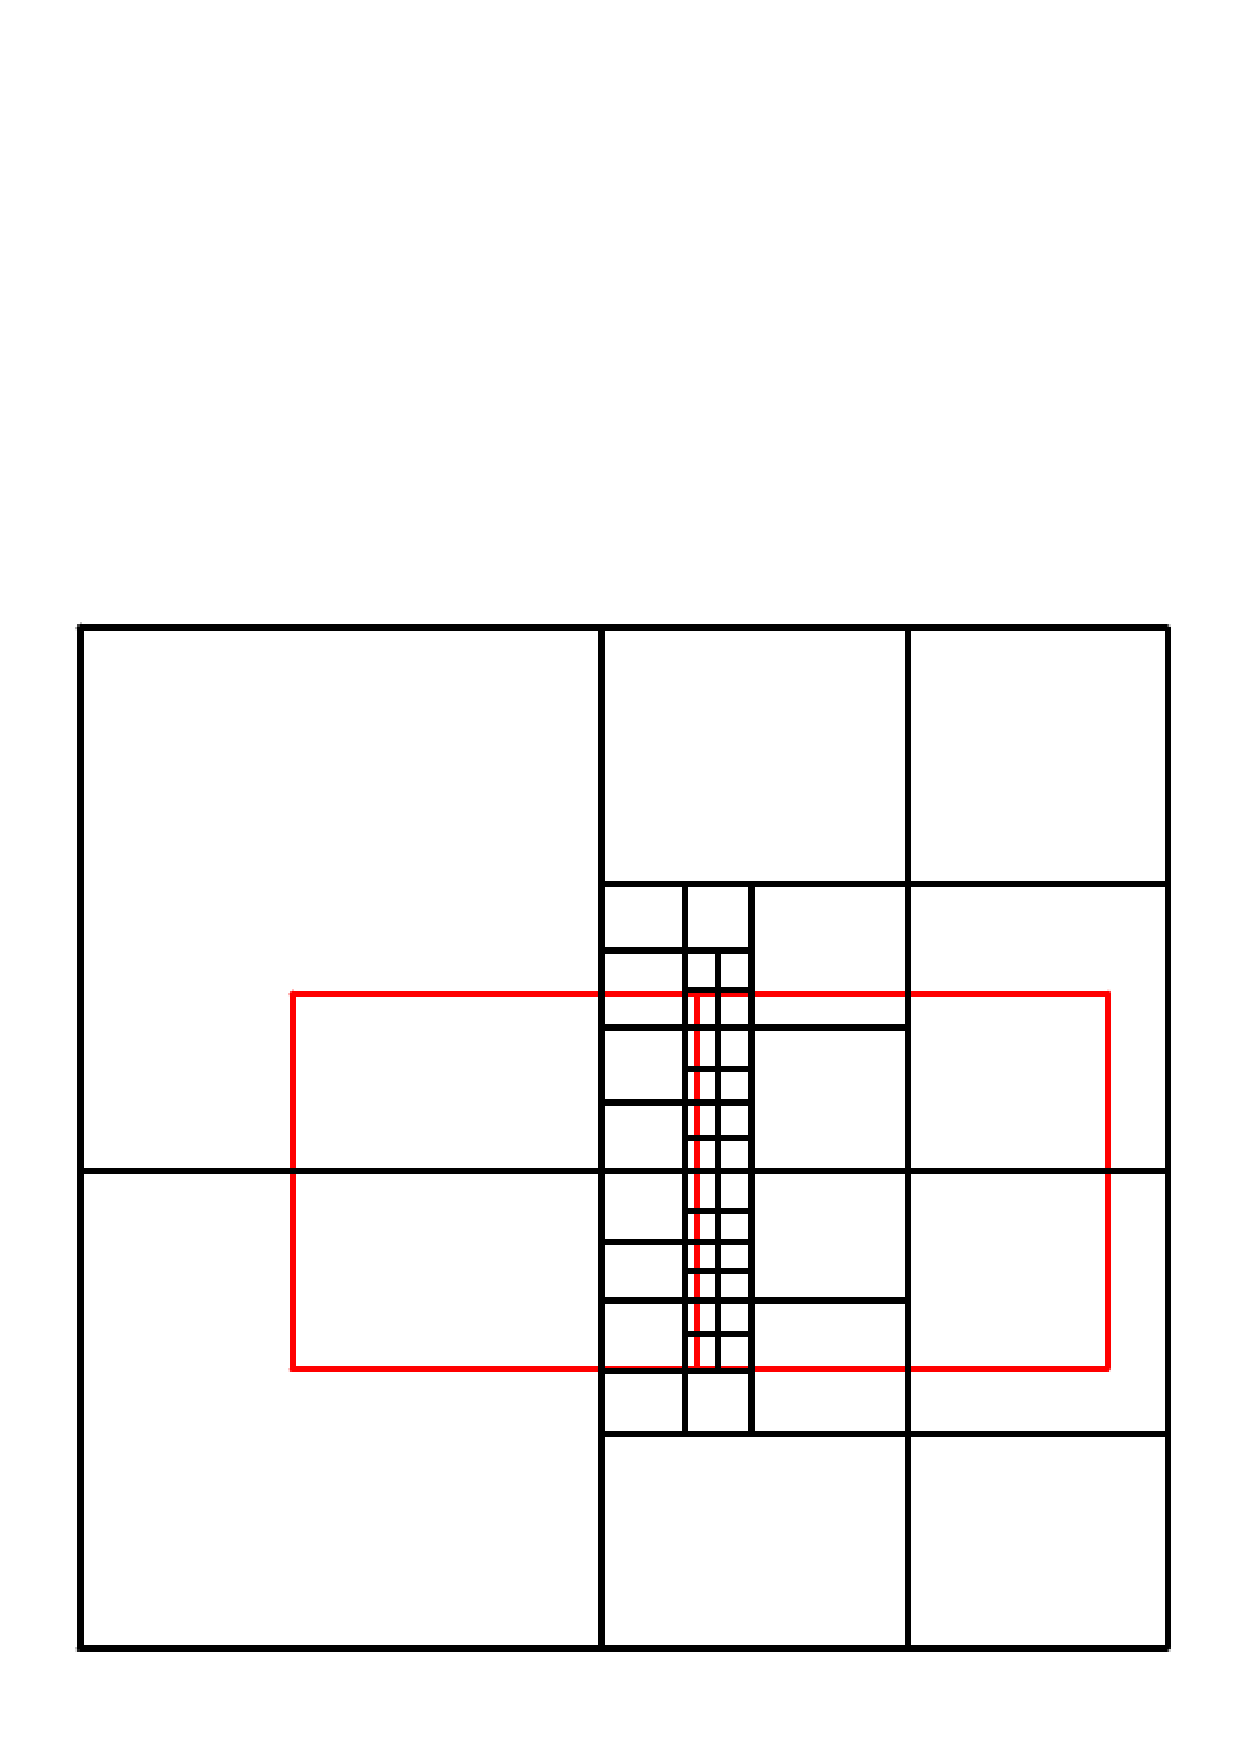
\includegraphics[width=0.50\textwidth]{img/SQT6}
        \end{center}
      \end{figure}
}

 \end{slide}
}
  %%%%%%%%%%%%%%%%%%%%%%%%%%%%%%%%%%%%%%%%%%%%%%%%%%%%%%%%%%%%%%%%%%%%%%%%%%%%
  \begin{slide}[Box]{Visualisation : R-Tree}
          \textbf{Exemple de représentation}
      \begin{figure}[t]

        \begin{center}
          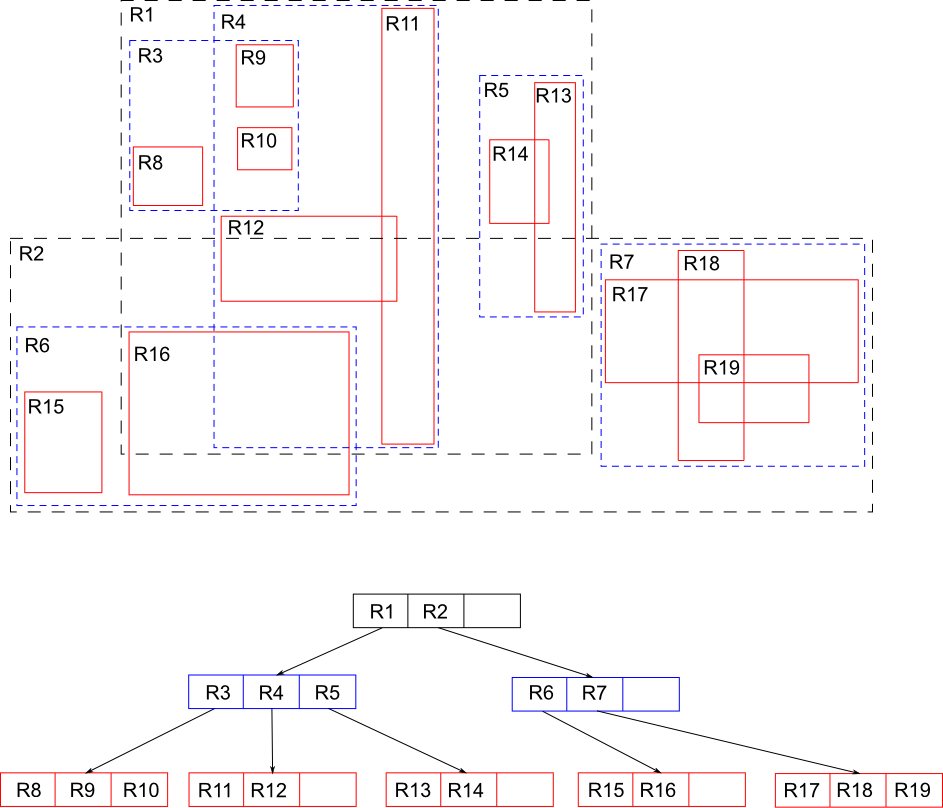
\includegraphics[width=0.55\textwidth]{img/rtree}
        \end{center}
      \end{figure}
  \end{slide}
  %%%%%%%%%%%%%%%%%%%%%%%%%%%%%%%%%%%%%%%%%%%%%%%%%%%%%%%%%%%%%%%%%%%%%%%%%%%%
\overlays{4}{
  \begin{slide}[Box]{Visualisation : R-Tree}
    \textbf{Description du R-Tree}
    \begin{Itemize}
      \fromSlide{2}{   \item Variante de l'arbre B}
      \fromSlide{3}{    \item Chaque nœud est un MBR de ces fils}
      \fromSlide{4}{  \item Chaque nœud contient entre $m$ et $M$ fils \\ avec $m \leq \frac{M}{2}$}
    \end{Itemize}
  \end{slide}
}
  %%%%%%%%%%%%%%%%%%%%%%%%%%%%%%%%%%%%%%%%%%%%%%%%%%%%%%%%%%%%%%%%%%%%%%%%%%%%

  \begin{slide}[Box]{Visualisation : R-Tree}
      \textbf{Hauteur de l'arbre et nombre de nœuds au pire cas}
    \begin{Itemize}
    \item Hauteur
      \begin{equation*}
        h_{max} = \left\lceil\log_{m} n\right\rceil - 1
      \end{equation*}
      \item Nombre de nœuds
      \begin{equation*}
        N_{noeuds}=\sum_{i=1}^{h_{max}}{\left\lceil\frac{n}{m^i}\right\rceil}
      \end{equation*}
    \end{Itemize}
  \end{slide}

  %%%%%%%%%%%%%%%%%%%%%%%%%%%%%%%%%%%%%%%%%%%%%%%%%%%%%%%%%%%%%%%%%%%%%%%%%%%%

\begin{slide}[Box]{Que reste-t-il à faire ?}
    \vspace{1cm}
    \begin{Itemize}
    \item Chercher la meilleure implémentation pour le R-Tree.
    \item Une étude approfondie pour prendre en compte la gestion des filtres.
    \item Trouver un moyen efficace de sauvegarde.
    \end{Itemize}
  \end{slide}

 \end{document}
